% !TEX program = xelatex

\documentclass[12pt, a4paper]{article}

\usepackage{fontspec}
\setmainfont[Ligatures=TeX]{Linux Libertine O}
\usepackage[left=2.5cm,right=2.5cm,top=2.5cm,bottom=2.5cm]{geometry}

\usepackage{amsmath,amsfonts,amssymb}


\usepackage{dirtytalk}
\usepackage{bookmark}
\usepackage{cite}
\usepackage{graphicx}
\usepackage{subcaption}
\usepackage{float}
\usepackage{siunitx}
\usepackage{color}
\usepackage{indentfirst}
\usepackage{cleveref}
\usepackage{booktabs}
\usepackage{tabularx}
\usepackage{wrapfig}

\usepackage[acronym]{glossaries}
\makeglossaries



\newcommand{\crefwithname}[1]{\cref{#1}: \nameref{#1}}

\graphicspath{{../assets/}}

\sloppy


\usepackage{setspace}
\onehalfspacing % 1.5 line spacing

\begin{document}

\begin{titlepage}
    \begin{figure}[H]
      \begin{center}
        \includegraphics[width=3cm]{auth.pdf}
        \label{fig:cover_auth_logo}
      \end{center}
    \end{figure}
    
    \centering
    \Large Αριστοτέλειο Πανεπιστήμιο Θεσσαλονίκης\\
    \Large Πολυτεχνική Σχολή\\
    \large Τμήμα Ηλεκτρολόγων Μηχανικών και Μηχανικών Υπλογιστών\\
    \large Τομέας Ηλεκτρονικής και Υπλογιστών

    
    \vspace{\fill}


    \Large Διπλωματική εργασία

    \vspace{\fill}
    
    \Large \textbf{Μάθηση πολλαπλών εργασιών στη μοντελοποίηση διαταραχών με εφαρμογή σε μονοκυτταρικά δεδομένα}
    

    \vspace{\fill}
    
    \Large Θεόδωρος Κατζάλης
    
    \large ΑΕΜ: 9282
    
    \vspace{\fill}
    \raggedright
    
    \begin{large}
    \begin{tabular}{ll}
    & \textbf{Επιβλέπων:} \\
    & Περικλής Μήτκας \\
    & Καθηγητής Αριστοτελείου Πανεπιστημίου Θεσσαλονίκης (Α.Π.Θ) \\
    & \\

    & \textbf{Συνεπιβλέπων:} \\
    & Φώτης Ε. Ψωμόπουλος \\
    & Ερευνητής στο Ινστιτούτο Εφαρμοσμένων Βιοεπιστημών (INAB) του\\
    & Εθνικού Κέντρου Έρευνας και Τεχνολογικής Ανάπτυξης (ΕΚΕΤΑ) \\

    \end{tabular}
    \end{large}
    
    \centering
    \vspace{\fill}
    \large Θεσσαλονίκη, Δεκέμβριος 2025
    
    \end{titlepage}
    
    % \begin{abstract}
    % abstract
    % \end{abstract}
    
    % \begin{abstract}
    % abstract
    % \end{abstract}
    
    % \thispagestyle{empty}
    
    
    % \section*{Ευχαριστίες}
    % \thispagestyle{empty}
    
    
    
    \clearpage
    

% \title{Τίτλος διπλωματικής}
% \author{Όνομα Επίθετο \\
% \href{mailto:empty@auth.gr}{empty@auth.gr}}
% \maketitle


% \begin{center}
% \textbf{\Large Acknowledgements}
% \end{center}


% \clearpage



\clearpage
\phantomsection
\addcontentsline{toc}{subsection}{Περίληψη}
\noindent
\textbf{\Large Περίληψη}
\newline

Οι προηγμένες μονοκυτταρικές τεχνολογίες έχουν δημιουργήσει νέες προοπτικές για την κατανόηση και αξιοποίηση των κυτταρικών αποκρίσεων σε διαταραχές, με σημαντικές εφαρμογές στο πεδίο της βιοιατρικής. Ωστόσο, η εγγενής πολυπλοκότητα των βιολογικών συστημάτων και οι τεχνικοί περιορισμοί των πειραματικών πρωτοκόλλων δημιουργούν προκλήσεις για πολλές από τις προτεινόμενες υπολογιστικές μεθόδους, δυσχεραίνοντας την αλγοριθμική ανάπτυξη των μηχανισμών διαταραχής. Η μάθηση πολλαπλών εργασιών (multi-task learning) αποτελεί μία από τις προσεγγίσεις που παραμένουν ανεξερεύνητες σε αυτό το πεδίο.
Στην παρούσα μελέτη, επιδιώκουμε να καλύψουμε αυτό το κενό, εξετάζοντας την προοπτική της στη μοντελοποίηση μονοκυτταρικών διαταραχών (single-cell multi-task learning). Αναπτύξαμε μια αρχιτεκτονική multi-task autoencoder, η οποία  έχει την δυνατότητα να προβλέπει για ένα σύνολο απο διαταραχές μονοκυτταρικά μεταγραφικά προφίλ εφαρμόζοντας μία από αυτές. Με τον τρόπο αυτόν επιτυγχάνει state-of-the-art αποτελέσματα, ενώ ταυτόχρονα επιδεικνύει μεγαλύτερη επεκτασιμότητα και αποδοτικότητα σε σύγκριση με τις υπάρχουσες μεθόδους. Ιδιαίτερο ενδιαφέρον θα είχε η περαιτέρω διερεύνηση και διαμόρφωση της αρχιτεκτονικής αυτής ως ένα θεωρητικό και αφηρημένο μοντέλο για την ταυτόχρονη επίλυση πολλαπλών σχετικών προβλημάτων στο πεδίο της μοντελοποίησης διαταρραχών και ευρύτερα της βιοπληροφορικής.

\vspace{1cm}
\noindent
\textbf{\Large Λέξεις κλειδιά}
\newline

\noindent
Μονοκυτταρική τεχνολογία, διαταραχή, μοντελοποίηση διαταραχής, μάθηση πολλαπλών εργασιών, autoencoder, βαθιά μάθηση


\clearpage
\phantomsection
\addcontentsline{toc}{subsection}{Abstract}
\noindent
\textbf{\Large Abstract}
\newline

Advanced single-cell technologies have provided new insights for the comprehension and utilization of cellular responses to perturbations, with significant potential for biomedicine. However, the inherent complexity of biological systems and the technical limitations of the experimental protocols present challenges for many proposed computational methods to algorithmically capture the perturbation mechanisms. Multi-task learning is one of the methods that have been left unexplored in this field. In this study, we aim to bridge this gap by unraveling its potential in single-cell perturbation modeling. We have developed a multi-task autoencoder architecture that predicts perturbed single-cell transcriptomic profiles for multiple perturbations. This method achieves state-of-the-art performance while exhibiting greater scalability and efficiency compared to existing methods. Further investigation and refinement of this architecture as a theoretical and abstract model for simultaneously solving multiple related problems in perturbation modeling and broader bioinformatics would be of particular interest.

\vspace{1cm}
\noindent
\textbf{\Large Keywords}
\newline

\noindent
Single-cell technology, perturbation, perturbation modeling, multi-task learning, autoencoder, deep learning


\clearpage
\phantomsection
\addcontentsline{toc}{subsection}{Ευχαριστίες}
\noindent
\textbf{\Large Ευχαριστίες}
\newline

Πρωτίστως, θα ήθελα να ευχαριστήσω θερμά τον επιβλέποντα καθηγητή αυτής της εργασίας, Περικλή Μήτκα, για την συνεργασία που μου επέτρεψε να έχω μαζί του και την ευκαιρία που μου έδωσε να εργαστώ σε αυτό το ερευνητικό πεδίο. Αυτή η συνεργασία μου έδωσε την δυνατότητα να ανακαλύψω μια αρκετά μοναδική σύνθεση ανάμεσα στην βιολογία και την μηχανική, επεκτείνοντας το πρόγραμμα σπουδών, η οποία μου κέντρισε το ενδιαφέρον και με ενέπνευσε να συνεχίσω την ενασχόληση μου σε αυτόν τον κλάδο στο μέλλον.

Επίσης, θα ήθελα να εκφράσω τις εγκάρδιες ευχαριστίες μου στην ομάδα βιοπληροφορικής του Ινστιτούτου Εφαρμοσμένων Βιοεπιστημών (ΙΝΕΒ) του Εθνικού Κέντρου Έρευνας και Τεχνολογικής Ανάπτυξης (ΕΚΕΤΑ) υπό την επίβλεψη του Φώτη Ε. Ψωμόπουλου, και συγκεκριμένα στον Γαβριηλίδη Γεώργιο, στον Βασιλείου Βασίλειο, και στην Ορφανού Άσπα. Η ομάδα με εισήγαγε στον χώρο της βιοπληροφορικής και με στήριξε πολυεπίπεδα καθ´ολη την διάρκεια της εργασίας μου, παρέχοντας τεχνογνωσία και αναπτύσσοντας επικοιδομητικές συζητήσεις, οι οποίες με βοήθησαν αμέριστα στον προσανατολισμό της έρευνάς μου.

Η εκπόνηση της εργασίας, ακόμη, θα ήταν ανέφικτη δίχως την πρόσβαση στους υπολογιστικούς πόρους του Ευρωπαϊκού Εργαστηρίου Μοριακής Βιολογίας (EMBL) της Χαϊδελβέργης. Θα ήθελα να ευχαριστήσω θερμά την Anna Kreshuk, επικεφαλής της ομάδας ανάλυσης βιολογικών εικόνων με την χρήση τεχνητής νοημοσύνης (Machine learning for bioimage analysis), για τη δυνατότητα που μου έδωσε να αποτελώ μέλος της ομάδας της ως μηχανικός λογισμικού στην πλατφόρμας ilastik\footnote{\url{https://www.ilastik.org/}}, και την παράλληλη παροχή πρόσβασης στην συστοιχία υπολογιστών για την επιτέλεση των πειραμάτων μου.

Τέλος, θα ήθελα να ευχαριστήσω την οικογένεια μου και τους φίλους μου για τη συναισθηματική υποστήριξη κατά την διάρκεια των σπουδών μου.

\clearpage

{
\renewcommand*\contentsname{Περιεχόμενα}
\hypersetup{linkcolor=black}
\tableofcontents
}

\thispagestyle{empty}

\clearpage
\phantomsection
\addcontentsline{toc}{subsection}{Κατάλογος Σχημάτων}
\renewcommand{\listfigurename}{Κατάλογος Σχημάτων}
\listoffigures

\clearpage
\phantomsection
\addcontentsline{toc}{subsection}{Κατάλογος Πινάκων}
\renewcommand{\listtablename}{Κατάλογος Πινάκων}
\listoftables


\clearpage
\phantomsection
\addcontentsline{toc}{subsection}{Ακρωνύμια}
\chapter{Ακρωνύμια και συντομογραφίες}

\begin{description}
  \item[LAN] Local Area Network
\end{description}

\printglossary[type=\acronymtype, title=Ακρωνύμια]
\clearpage


% I have mentioned that scvidr is a multi-task model. Thus, maybe I have to rephrase it since there were some attempts but not fully dedicated to explore the multi-task as a learning paradigm per se.

\section{Εισαγωγή}


Η εφαρμογή των αρχών και των τεχνικών της επιστήμης των υπολογιστών αποτελούν πλέον αναπόσπαστο κομμάτι της βιολογικής έρευνας. Η χρήση υπολογιστικών μεθόδων και η κατασκευή εργαλείων για την μελέτη και την ανάλυση των βιολογικών δεδομένων, πεδίο γνωστό και ως βιοπληροφορική, ξέκινησε ήδη απο το 1960 έχοντας ως αφετηρία την ανάλυση πρωτεϊνικών αλληλουχιών. Πλεόν, την σύγχρονη εποχή, χάρη στην τεχνολογική πρόοδο, όπως της τεχνολογίας "επόμενης γενιάς αλληλούχισης" (next-generation sequencing, NGS), το πεδίο εκτείνεται μέχρι και την ιχνηλάτηση της αλληλουχίας του DNA σε μεγάλη κλίμακα \cite{gauthier2019brief}. Έτσι, η μηχανική μάθηση βρίσκει πρόσφορο έδαφος για την ανάπτυξη αλγορίθμων που μπορούν να αναλύσουν και να ερμηνεύσουν τα τεράστια αυτά σύνολα δεδομένων \cite{libbrecht2015machine}.


\subsection{Συνοπτική περιγραφή του προβλήματος}

Η εμφάνιση των μονοκυτταρικών τεχνολογιών έχει καταστήσει δυνατή τη μελέτη της βιολογικής ετερογένειας σε κυτταρική ανάλυση, ανοίγοντας νέους δρόμους για την κατανόηση των κυτταρικών μηχανισμών και των αποκρίσεών τους σε διαταραχές.
Ωστόσο, ο χώρος των διαταραχών είναι ευρύς, και η πειραματική διερεύνηση όλων των πιθανών συνδυασμών θα ήταν ανέφικτη και δαπανηρή \cite{heumos2023best, kana2023generative}.
Αυτό έχει οδηγήσει στην ανάπτυξη υπολογιστικών μεθόδων για τη μοντελοποίηση του χώρου αυτού, επιτρέποντας την εξαγωγή συμπερασμάτων σε καινούρια σενάρια μέσω in silico πειραματισμού διευρύνοντας τον χρονοβόρο και δαπανηρό in vitro και in vivo πειραματισμό.
Το πεδίο που ασχολείται με την αποκωδικοποίηση και πρόβλεψη των επιδράσεων εξωτερικών ερεθισμάτων (γονιδιακές απαλοιφές, δοσολογίες φαρμάκων, μεταβολές θερμοκρασίας κ.ά.) αναφέρεται ως μοντελοποίηση διαταραχών (perturbation modeling), και διαδραματίζει κρίσιμο ρόλο στην ανακάλυψη μηχανισμών ασθενειών και στον εντοπισμό θεραπευτικών στόχων \cite{jiMachineLearningPerturbational2021}.

\subsection{Στόχος της διπλωματικής}

Η πολυπλοκότητα της βιολογικής απόκρισης σε διαταραχές θα μπορούσε να αποδομηθεί σε επιμέρους, σχετικούς στόχους για την απλοποίηση και την καλύτερη κατανόηση της διαδικασίας.
H μάθηση πολλαπλών εργασιών (Multi-task learning) είναι μία τεχνική μηχανικής μάθησης, η οποία θα μπορούσε να αξιοποιήσει αυτήν την αποδόμηση, καθώς επιτρέπει την ταυτόχρονη εκμάθηση πολλαπλών σχετικών εργασιών, ενισχύοντας τη γενίκευση και την απόδοση μέσω της κοινής χρήσης αναπαραστάσεων \cite{ruderOverviewMultiTaskLearning2017}.
Έτσι, αυτή η τεχνική θα μπορούσε να είναι μια πολλά υποσχόμενη προσέγγιση για την αντιμετώπιση των προκλήσεων που παρουσιάζονται στην μοντελοποίηση μονοκυτταρικών διαταραχών.
Ωστόσο, παρά τα πλεονεκτήματα που προσφέρει, η εφαρμογή της σε αυτό το πεδίο παραμένει ανεξερεύνητη. Στην παρούσα εργασία, επιδιώκουμε να καλύψουμε αυτό το κενό, εξετάζοντας την προοπτική της.


\subsection{Μεθοδολογία}

Αρχικά επιχειρήσαμε να διερευνήσουμε ποιές εργασίες θα μπορούσαν να αποδομηθούν από την κύρια εργασία της πρόβλεψης διαταραχών, ώστε να αξιοποιηθεί η μάθηση πολλαπλών εργασιών. Στη συνέχεια, εστιάσαμε σε εφαρμογές μονοκυτταρικών δεδομένων, και συγκεκριμένα στην πρόβλεψη γονιδιακής έκφρασης μετά από μια δαταραχή.

Για να αξιοποιήσουμε την τεχνική της μάθησης πολλαπλών εργασιών, αναπτύξαμε μια αρχιτεκτονική multi-task autoencoder, η οποία για ένα σύνολο απο διαταραχές έχει την δυνατότητα να προβλέπει μονοκυτταρικά μεταγραφικά προφίλ εφαρμόζοντας μία από αυτές. Η διαταραχή μοντελοποιήθηκε ως ένα διάνυσμα, το οποίο κωδικοποιεί τον τύπο της διαταραχής και ενσωματώνεται στην αρχιτεκτονική του autoencoder μέσω FiLM layers \cite{dumoulin2018feature-wise}, η οποία αποτελεί έναν τύπο αθροιστικού και πολλπλασιαστικού μετασχηματισμού που εφαρμόζεται σε κάθε κόμβο του επιπέδου (layer) του δικτύου που μας ενδιαφέρει.

Η αξιολόγηση του μοντέλου πραγματοποιήθηκε για τρία διαφορετικά σενάρια, συγκριτικά με state-of-the-art μεθόδους μονοκυτταρικής πρόβλεψης μεταγραφικών προφίλ μετά από διαταραχή. 


\subsection{Περιεχόμενα}

Στο κεφάλαιο 2 παρουσιάζεται το θεωρητικό υπόβαθρο της εργασίας. Στο κεφάλαιο 3 περιγράφεται ο αλγόριθμος. Στο κεφάλαιο 4 παρουσιάζονται τα αποτελέσματα των πειραμάτων που υλοποιήθηκαν για τρία διαφορετικά σενάρια, μονή διαταραχή, πολλαπλές διαταραχές και μονή διαταραχή μεταξύ διαφορετικών ειδών. Τέλος, στο κεφάλαιο 5 αναλύονται τα αποτελέσματα των πειραμάτων, γίνεται σύγκριση, δίνονται τα συμπεράσματα της συνολικής διαδικασίας καθώς και οι μελλοντικοί στόχοι που μπορούν τα τεθούν για περεταίρω επεκτάσεις και ακολουθεί η βιβλιογραφία που χρησιμοποιήθηκε για τη συγγραφή αλλά και την υλοποίηση της εργασίας αυτής.

\clearpage

\section{Θεωρητικό υπόβαθρο}

Τα σύνολα δεδομένων που χρησιμοποιούνται για τη μοντελοποίηση διαταραχών είναι συχνά ιδιαίτερα θορυβώδη και αραιά, λόγω των εγγενών περιορισμών των μονοκυτταρικών τεχνολογιών. Για παράδειγμα, είναι πιθανό να προκύψουν φαινόμενα dropout, οδηγώντας σε μεγάλο αριθμό μηδενικών τιμών στα προφίλ έκφρασης, ως αποτέλεσμα της αδυναμίας ανίχνευσης χαμηλών επιπέδων γονιδιακής έκφρασης. Επιπλέον, τα δεδομένα είναι υψηλής διαστασιμότητας, αποτελούμενα συνήθως από χιλιάδες κύτταρα που έχουν μελετηθεί ως προς εκατοντάδες ή και χιλιάδες χαρακτηριστικά (π.χ. επίπεδα γονιδιακής έκφρασης στη μεταγραφωμική), γεγονός που επιτρέπει λεπτομερή ανάλυση των κυτταρικών αποκρίσεων \cite{jiMachineLearningPerturbational2021}. Η ίδια η απόκριση στις διαταραχές είναι μη γραμμική και περίπλοκη, εξαρτώμενη όχι μόνο από τη φύση της διαταραχής, αλλά και από το κυτταρικό περιβάλλον, συμπεριλαμβανομένου του τύπου κυττάρου, του μικροπεριβάλλοντος, του γενετικού υποβάθρου και της χρονικής δυναμικής \cite{gavriilidisMinireviewPerturbationModelling2024}.

Οι μέθοδοι μηχανικής μάθησης —ιδίως η βαθιά μάθηση (deep learning)— έχουν δείξει σημαντικές δυνατότητες στην αντιμετώπιση αυτής της πολυπλοκότητας, αξιοποιώντας τη γενετική τους ικανότητα, η οποία καθίσταται εφικτή χάρη στη ραγδαία αύξηση των δεδομένων μονοκυτταρικών υψηλής διαμέτρησης (high-throughput) \cite{gavriilidisMinireviewPerturbationModelling2024}. Πιο συγκεκριμένα, υπάρχει αυξανόμενο ενδιαφέρον για την αξιοποίηση των μεγάλων γλωσσικών μοντέλων (large language models, LLMs) στον τομέα αυτό. Μια πρόσφατη επισκόπηση από τους Szalata et al. \cite{szalata2024transformers} υπογραμμίζει αυτήν την προσέγγιση ως μια πολλά υποσχόμενη, αν και ακόμη ανώριμη, ερευνητική κατεύθυνση. Τα κύρια προβλήματα περιλαμβάνουν την απουσία τυποποιημένων πλαισίων αξιολόγησης, αστάθειες στα μοντέλα, ανεπαρκώς ποικιλόμορφα σύνολα δεδομένων και την έλλειψη διαδοχικής δομής ανάλογης με τα positional embeddings που χρησιμοποιούνται στην επεξεργασία φυσικής γλώσσας.
Αντίθετα, οι αρχιτεκτονικές autoencoders και οι παραλλαγές τους έχουν ήδη επιδείξει ισχυρές επιδόσεις, ξεπερνώντας τους transformers \cite{szalata2024transformers}, ενώ προσφέρουν σημαντικά πλεονεκτήματα όσον αφορά την αποδοτικότητα πόρων και τη μειωμένη υπολογιστική πολυπλοκότητα.

Βασιζόμενες στην κεντρική αρχή της βαθιάς μάθησης, γνωστή ως manifold hypothesis, οι αρχιτεκτονικές autoencoder στοχεύουν στην εκμάθηση μιας αναπαράστασης των δεδομένων σε μικρό αριθμό διαστάσεων που αποτυπώνει τη θεμελιώδη δομή της απόκρισης στη διαταραχή. Αυτό επιτυγχάνεται μέσω της αρχιτεκτονικής κωδικοποιητή-αποκωδικοποιητή (encoder–decoder), όπου ο κωδικοποιητής συμπιέζει τα δεδομένα εισόδου σε χώρο μικρότερης διάστασης, ενώ ο αποκωδικοποιητής επιχειρεί να ανακατασκευάσει τα αρχικά δεδομένα. Αυτή η συμπίεση μπορεί να παράγει βιολογικά σημαντικά χαρακτηριστικά, οδηγώντας σε πιο ερμηνεύσιμη και αποδοτική αναπαράσταση των δεδομένων, χρήσιμη για επακόλουθες εργασίες όπως η ανίχνευση αποκρίσεων εκτός του παρατηρούμενου χώρου (out-of-distribution, OOD) \cite{gavriilidisMinireviewPerturbationModelling2024}.

Ωστόσο, η μη γραμμικότητα των μοντέλων βαθιάς μάθησης παρουσιάζει μια επιπλέον πρόκληση όσον αφορά την ισορροπία μεταξύ ακρίβειας πρόβλεψης και ερμηνευσιμότητας \cite{kana2023generative}. Αυτή η αντιστάθμιση παραμένει κομβικό σημείο για το πεδίο, και πολλές πρόσφατες προσπάθειες στοχεύουν στην αντιμετώπισή της μέσω αιτιοκρατικών προσεγγίσεων μηχανικής μάθησης, όπως τα GRouNdGAN, sVAE+ και graphVCI \cite{gavriilidisMinireviewPerturbationModelling2024}. Άλλες ερμηνεύσιμες προσεγγίσεις περιλαμβάνουν τη χρήση τιμών SHAP από το UnitedNet \cite{tangExplainableMultitaskLearning2023}, integrated gradients από το PerturbNet \cite{yuPerturbNetPredictsSinglecell2022}, καθώς και την προσέγγιση της συνάρτησης του μη ερμηνεύσιμου μη γραμμικού αποκωδικοποιητή μέσω sparse ridge regression, όπως παρουσιάζεται στο scVIDR \cite{kanaGenerativeModelingSinglecell2023}.

Επιπλέον περιορισμοί στα δεδομένα, όπως τα batch effects και οι συγχυτικοί συν-παράγοντες (confounding covariates), επηρεάζουν επίσης την ακρίβεια πρόβλεψης. Για την αντιμετώπιση αυτών των ζητημάτων και τη βελτίωση της γενίκευσης, πρόσφατες μελέτες επικεντρώνονται σε ενοποιητικές μονοκυτταρικές προσεγγίσεις omics ανάλυσης (integrative single-cell omics), συμπεριλαμβανομένης της ενσωμάτωσης χωρικών δεδομένων. Ο στόχος είναι η εκμάθηση μιας αναπαράστασης με μικρό αριθμό διαστάσεων που απομονώνει το ουσιώδες βιολογικό πλαίσιο, απαλλάσσοντάς το από τεχνικές παραλλαγές.

\subsection{Μάθηση πολλαπλών διεργασιών (Multi-task learning)}

Η μάθηση πολλαπλών εργασιών (\gls{mlt}) αποτελεί ένα παράδειγμα παραδείγματος μηχανικής μάθησης, στο οποίο ένα ενιαίο μοντέλο εκπαιδεύεται ώστε να εκτελεί ταυτόχρονα πολλαπλές, σχετικές μεταξύ τους εργασίες. Η κεντρική ιδέα είναι ότι, μέσω της κοινής χρήσης αναπαραστάσεων μεταξύ των εργασιών, το μοντέλο μπορεί να γενικεύσει καλύτερα σε σύγκριση με το αν κάθε εργασία μαθαίνονταν απομονωμένα. Η προσέγγιση αυτή αντλεί έμπνευση από τη μάθηση και τη γνωστική λειτουργία του ανθρώπου, όπου η αναλογία παίζει κεντρικό ρόλο στη μεταφορά γνώσης μεταξύ διαφορετικών γνωστικών περιοχών \cite{hofstadter2001analogy, zhangSurveyMultiTaskLearning2021}.
Από τη σκοπιά της μηχανικής μάθησης, μπορούμε να τη θεωρήσουμε ως μια μορφή επαγωγικής προκατάληψης (inductive bias): κατευθύνει το μοντέλο να προτιμά υποθέσεις που εξηγούν περισσότερες από μία εργασίες, ανάλογα με τη λογική της L1 κανονικοποίησης, η οποία οδηγεί σε προτίμηση για αραιές λύσεις \cite{ruderOverviewMultiTaskLearning2017}. Ο βαθμός ωφέλειας εξαρτάται από τη σχέση μεταξύ των εργασιών· όταν οι εργασίες δεν είναι στενά συνδεδεμένες, μπορεί να προκύψει αρνητική μεταφορά (negative transfer), κατά την οποία η μάθηση μιας εργασίας επιδρά αρνητικά στην επίδοση μιας άλλης \cite{standleyWhichTasksShould2020}. Συνεπώς, η κατανόηση των σχέσεων μεταξύ των εργασιών και ο σχεδιασμός κατάλληλων κοινών αρχιτεκτονικών αποτελούν κρίσιμους παράγοντες για την επιτυχία της \gls{mlt}.

Ένα από τα αρχικά κίνητρα της μάθησης πολλαπλών εργασιών είναι η έμμεση αύξηση δεδομένων (implicit data augmentation), μέσω του συνδυασμού πηγών πληροφορίας από διαφορετικές εργασίες, ώστε να μετριαστεί το πρόβλημα της έλλειψης δεδομένων. Αυτό είναι ιδιαίτερα σχετικό στα μονοκυτταρικά πρωτόκολλα πολλαπλών omics (single-cell multi-omics) \cite{caoScButterflyVersatileSinglecell2024}, όπου τα δεδομένα είναι περιορισμένα λόγω της πολυπλοκότητας και του κόστους των πειραματικών διαδικασιών. Παρόμοια οφέλη παρατηρούνται και στα μονοκυτταρικά σύνολα δεδομένων μονοτροπίας (single-cell single modality), όπου τα δεδομένα είναι περιορισμένα για συγκεκριμένο αριθμό διαταραχών.

Άλλα πλεονεκτήματα της \gls{mlt} περιλαμβάνουν την πρόληψη της υπερεκπαίδευσης (overfitting) και τη μείωση του εξαρτώμενου από τα δεδομένα θορύβου κάθε εργασίας. Ο θόρυβος μπορεί να αποκρύψει τα υποκείμενα πρότυπα, καθιστώντας δύσκολη τη μάθηση ουσιαστικών αναπαραστάσεων. Ο συνδυασμός δεδομένων από πολλαπλές εργασίες παρέχει πρόσθετα στοιχεία, επιτρέποντας στο μοντέλο να διακρίνει τα σημαντικά χαρακτηριστικά από τα άσχετα, οδηγώντας έτσι σε πιο ανθεκτικά και γενικεύσιμα χαρακτηριστικά \cite{ruderOverviewMultiTaskLearning2017}. Αυτό είναι ιδιαίτερα σημαντικό στη μοντελοποίηση μονοκυτταρικών διαταραχών, όπου τα δεδομένα είναι συχνά θορυβώδη και αραιά, λόγω dropout γεγονότων και άλλων τεχνικών περιορισμών.

Όσον αφορά την επιλογή αρχιτεκτονικής στη \gls{mlt}, πρέπει να εξεταστεί ο τρόπος αλληλεπίδρασης των εργασιών, μια έννοια γνωστή ως conditioning \cite{dumoulin2018feature-wise}. Στο πλαίσιο της βαθιάς μάθησης, οι δύο πιο διαδεδομένες προσεγγίσεις είναι η σκληρή (hard) και η ήπια (soft) κοινή χρήση παραμέτρων.
Στην σκληρή κοινή χρήση, το μοντέλο μοιράζεται ένα κοινό σύνολο παραμέτρων για όλες τις εργασίες, διατηρώντας όμως ξεχωριστή κεφαλή (head) για καθεμία (\cref{fig:hard}). Αυτή η προσέγγιση είναι η πιο συνηθισμένη και προτιμάται όταν οι εργασίες είναι στενά συνδεδεμένες, καθώς επιτρέπει πιο αποδοτική μάθηση και μειώνει τον κίνδυνο υπερεκπαίδευσης.
Αντίθετα, στην ήπια κοινή χρήση παραμέτρων, κάθε εργασία διαθέτει το δικό της σύνολο παραμέτρων, αλλά αυτές ενθαρρύνονται να είναι παρόμοιες μέσω κανονικοποίησης (\cref{fig:soft}). Η προσέγγιση αυτή είναι πιο κατάλληλη για λιγότερο συσχετισμένες εργασίες, καθώς προσφέρει μεγαλύτερη ευελιξία στην εκμάθηση εξειδικευμένων αναπαραστάσεων ανά εργασία, ενώ ταυτόχρονα είναι λιγότερο επιρρεπής σε αρνητική μεταφορά \cite{ruderOverviewMultiTaskLearning2017}.

\begin{figure}[h!]
    \centering
    \begin{subfigure}[t]{0.48\textwidth}
        \centering
        \includegraphics[width=.6\textwidth]{hard.png}
    \caption{Σκληρή κοινή χρήση παραμέτρων}
        \label{fig:hard}
    \end{subfigure}
    \hfill
    \begin{subfigure}[t]{0.48\textwidth}
        \centering
        \includegraphics[width=\textwidth]{soft.png}
    \caption{Ήπια κοινή χρήση παραμέτρων}
        \label{fig:soft}
    \end{subfigure}
    \caption{Προσαρμογή εργασιών (Task conditioning) \cite{ruderOverviewMultiTaskLearning2017}}
    \label{}
\end{figure}

Μια άλλη προσέγγιση για την προσαρμογή (conditioning) των εργασιών είναι η οικογένεια των μετασχηματισμών κατά χαρακτηριστικό (feature-wise transformations). Στην προσέγγιση αυτή μπορούν να εφαρμοστούν τρεις διαφορετικοί τύποι μετασχηματισμού:
α) συνένωση (concatenation),
β) πρόσθεση (addition), και
γ) πολλαπλασιασμός (multiplication).

Οι μετασχηματισμοί αυτοί μπορούν να εφαρμοστούν ανά επίπεδο (layer-wise), προσφέροντας μεγαλύτερη ευελιξία στον τρόπο με τον οποίο οι εργασίες ενσωματώνονται στο μοντέλο. Μπορούν να εισαχθούν είτε στην αρχική είσοδο της αρχιτεκτονικής είτε σε μεταγενέστερο στάδιο της διαδικασίας δημιουργίας (generation process).

Στην περίπτωση της συνένωσης, για μια αναπαράσταση της εργασίας $z$ (π.χ. κωδικοποιημένη σε μορφή one-hot), η είσοδος ενός επιπέδου συνενώνεται με το $z$, και το αποτέλεσμα υποβάλλεται σε γραμμικό μετασχηματισμό.
Αντίθετα, στις περιπτώσεις της πρόσθεσης και του πολλαπλασιασμού, η αναπαράσταση προσαρμογής (conditioning representation) υφίσταται πρώτα γραμμικό μετασχηματισμό και στη συνέχεια προστίθεται ή πολλαπλασιάζεται με την είσοδο, αντίστοιχα.

Σε όλες αυτές τις μεθόδους, οι πράξεις εφαρμόζονται ανά χαρακτηριστικό (element-wise), εξ ου και η ονομασία μετασχηματισμοί κατά χαρακτηριστικό (feature-wise transformations) \cite{dumoulin2018feature-wise}.

\begin{figure}[h!]
    \centering
    \begin{subfigure}[t]{0.48\textwidth}
        \centering
        \includegraphics[width=\textwidth]{concat.png}
    \caption{Συνένωση}
        \label{}
    \end{subfigure}
    \hfill
    \begin{subfigure}[t]{0.48\textwidth}
        \centering
        \includegraphics[width=\textwidth]{add.png}
    \caption{Πρόσθεση}
        \label{}
    \end{subfigure}
    \begin{subfigure}[b]{.48\textwidth}
        \centering
        \includegraphics[width=\textwidth]{mul.png}
    \caption{Πολλαπλασιασμός}
        \label{}
    \end{subfigure}    
    \caption{Μετασχηματισμοί ανά χαρακτηριστικό \cite{ruderOverviewMultiTaskLearning2017}}
    \label{}
\end{figure}

Γενικότερα, οι μέθοδοι μάθησης πολλαπλών εργασιών (\gls{mlt}) μπορούν να κατηγοριοποιηθούν με βάση διάφορες διαστάσεις, όπως το παράδειγμα μάθησης (π.χ. επιβλεπόμενη ή μη επιβλεπόμενη μάθηση), τον τύπο των εργασιών (π.χ. ταξινόμηση ή παλινδρόμηση) και τη φύση του χώρου εισόδου.  
Στην παρούσα εργασία εστιάζουμε κυρίως σε επιβλεπόμενες εργασίες, οι οποίες αποτελούν και το πλέον μελετημένο πλαίσιο στη βιβλιογραφία της \gls{mlt} \cite{zhangSurveyMultiTaskLearning2021}.  

Όπως θα παρουσιαστεί στην \crefwithname{sec:method}, η βασική εργασία που εξετάζουμε αφορά την πρόβλεψη των προφίλ γονιδιακής έκφρασης μετά από μια διαταραχή, η οποία μπορεί να διατυπωθεί ως πρόβλημα παλινδρόμησης.  
Η είσοδος αποτελείται από το βασικό προφίλ γονιδιακής έκφρασης ενός κυττάρου (ή το λεγόμενο “vehicle” προφίλ), ενώ η έξοδος αντιστοιχεί στο προφίλ έκφρασης μετά την εφαρμογή της διαταραχής.  
Η ίδια η διαταραχή αναπαρίσταται μέσω ενός διανύσματος συνθηκών (condition vector), το οποίο μπορεί απλά να υλοποιηθεί ως one-hot κωδικοποίηση που προσδιορίζει τον τύπο της διαταραχής που εφαρμόστηκε στο κύτταρο.  

Τυπικά, για επιβλεπόμενες εργασίες που μοιράζονται τον ίδιο χώρο εισόδου, μπορούμε να ορίσουμε ένα σύνολο από $m$ εργασίες μάθησης $\{T_{i}\}_{i=1}^m$, και για καθεμία από αυτές το αντίστοιχο σύνολο δεδομένων $\mathcal{D}_i$, το οποίο περιέχει $n_i$ δείγματα:
\[
\mathcal{D}_i = \left\{(x_j^i, y_j^i)\right\}_{j=1}^{n_i}
\]
όπου $x_j^i$ είναι το $j$-οστό δείγμα εισόδου και $y_j^i$ η αντίστοιχη ετικέτα εξόδου του.  

Η συνάρτηση κόστους (loss) για την $i$-οστή εργασία μπορεί να διατυπωθεί ως:
\[
\mathcal{L}_i(\{\theta_i, \theta_{sp}\}, \mathcal{D}_i),
\]
όπου $\theta_i$ αντιστοιχούν στις ειδικές παραμέτρους της εργασίας, ενώ $\theta_{sp}$ στις κοινές παραμέτρους μεταξύ όλων των εργασιών.  

Ο στόχος της \gls{mlt} είναι η εκμάθηση ενός συνόλου παραμέτρων $\theta$ που ελαχιστοποιεί τη συνολική απώλεια για όλες τις εργασίες, δηλαδή:
\[
\theta = \arg\min_{\theta} \sum_{i=1}^m \mathcal{L}_i(\theta_i, \mathcal{D}_i),
\]
όπου
\[
\theta = \{\theta_{sp}, \theta_1, \dots, \theta_m\}
\]
αντιπροσωπεύει το πλήρες σύνολο των παραμέτρων του μοντέλου.

\subsection{Μοντελοποίηση διαταρραχών (Perturbation modeling)}

Στο πεδίο της μοντελοποίησης διαταραχών μπορούν να διακριθούν τέσσερις κύριοι ερευνητικοί στόχοι \cite{gavriilidisMinireviewPerturbationModelling2024, jiMachineLearningPerturbational2021, heumos2023best}.

\begin{itemize}
\setlength\itemsep{0.2em}
    \item Ο πρώτος αφορά την πρόβλεψη άγνωστων omics υπογραφών και φαινοτυπικών μεταβολών μετά από την εφαρμογή μιας διαταραχής.\footnote{Στην περίπτωση χημικών διαταραχών, ο όρος “διαταραχή” αναφέρεται στο συγκεκριμένο φάρμακο που εφαρμόζεται. Ωστόσο, για τους σκοπούς της εργασίας \gls{ood}, μια αλλαγή στη δοσολογία του ίδιου φαρμάκου θεωρείται επίσης διακριτή διαταραχή. Στην παρούσα μελέτη, κάθε μοναδικός συνδυασμός φαρμάκου και δοσολογίας αντιμετωπίζεται ως ξεχωριστή διαταραχή.}
Η πρόβλεψη αυτή μπορεί να εφαρμοστεί είτε σε κυτταρικές σειρές (bulk omics), είτε σε μεμονωμένα κύτταρα (single-cell omics) και αποτελεί τον πρωταρχικό στόχο, γνωστό και ως εκτός κατανομής πρόβλεψη (out-of-distribution prediction, OOD).
Όσον αφορά τις omics υπογραφές, το scGen αποτελεί ένα γνωστό μοντέλο αναφοράς για την πρόβλεψη προφίλ μεταγραφωμικής σε διαταραγμένα μονοκύτταρα.
Στην περίπτωση των φαινοτυπικών αλλαγών, αυτές μπορεί να αφορούν, για παράδειγμα, τη βιωσιμότητα των κυττάρων ως συνάρτηση της δοσολογίας ενός φαρμάκου, η οποία συνήθως ποσοτικοποιείται μέσω των τιμών IC50.
Ένα χαρακτηριστικό παράδειγμα αποτελεί το DeepDSC \cite{li2019deepdsc}, ένα βαθύ νευρωνικό δίκτυο που προβλέπει την ευαισθησία καρκινικών κυτταρικών σειρών σε φάρμακα, με βάση τα προφίλ γονιδιακής έκφρασης και έναν περιγραφέα χημικής ένωσης.
Ο περιγραφέας αυτός βασίζεται στα αποτυπώματα Morgan (Morgan fingerprints),\footnote{Τα αποτυπώματα Morgan, γνωστά και ως extended-connectivity fingerprints (ECFP), είναι ένας τύπος μοριακών αποτυπωμάτων που χρησιμοποιούνται στη χημειοπληροφορική για την αναπαράσταση της δομής μορίων σε μορφή κατάλληλη για υπολογιστική επεξεργασία. Κωδικοποιούν τα δομικά χαρακτηριστικά ενός μορίου σε ένα δυαδικό διάνυσμα \cite{morgan1965generation}.}
τα οποία αποτυπώνουν τη μονοδιάστατη και δισδιάστατη δομή της ένωσης.
    \item Ο δεύτερος στόχος αφορά την πρόβλεψη του μηχανισμού δράσης μιας διαταραχής (mode of action).
Αυτό συνεπάγεται την αναγνώριση των σηματοδοτικών οδών και των συγκεκριμένων πρωτεϊνών-στόχων που ενεργοποιούνται ή αναστέλλονται ως απόκριση σε μια δεδομένη διαταραχή.
Η κατανόηση των πρωτεϊνών με τις οποίες αλληλεπιδρά ένα φάρμακο, καθώς και της αλληλουχίας των μοριακών γεγονότων που προκαλεί, είναι θεμελιώδης για την ανακάλυψη και επαναστόχευση φαρμάκων (drug discovery and repurposing).
Το DeepDTAGen \cite{shah2025deepdtagen} είναι ένα πολυ-εργασιακό μοντέλο (multi-task model) σχεδιασμένο για να αντιμετωπίζει αυτή την πρόκληση.
Προβλέπει την ισχύ δέσμευσης (binding affinity) μεταξύ ενός φαρμάκου και μιας πρωτεΐνης-στόχου, ενώ παράγει και νέους υποψήφιους χημικούς συνδέτες, οι οποίοι αναπαρίστανται με αλφαριθμητικές συμβολοσειρές SMILES\footnote{Το ακρωνύμιο SMILES προέρχεται από το Simplified Molecular Input Line Entry System. Πρόκειται για μια συμβολική, κειμενοστραφή αναπαράσταση μοριακών δομών. Για παράδειγμα, η αιθανόλη (CH₃CH₂OH) μπορεί να αναπαρασταθεί ως η συμβολοσειρά “CCO”.}, προσαρμοσμένες σε έναν δεδομένο πρωτεϊνικό στόχο.
    \item Ο τρίτος στόχος είναι η πρόβλεψη αλληλεπιδράσεων διαταραχών, ένα πεδίο με ιδιαίτερη σημασία για συνδυαστικές θεραπείες.
Ο σκοπός είναι η πρόβλεψη του τρόπου με τον οποίο διαφορετικές διαταραχές αλληλεπιδρούν μεταξύ τους — κρίσιμο ζήτημα για την κατανόηση αλληλεπιδράσεων φαρμάκων (drug-drug interactions) και πιθανών παρενεργειών.
Αυτό περιλαμβάνει, για παράδειγμα, την πρόβλεψη του αν δύο φάρμακα θα παρουσιάσουν συνεργιστικά ή ανταγωνιστικά αποτελέσματα όταν χορηγηθούν μαζί.
Το μοντέλο DeepSynergy προβλέπει έναν δείκτη συνεργίας (synergy score), έχοντας ως είσοδο τα προφίλ γονιδιακής έκφρασης μιας κυτταρικής σειράς και τους χημικούς περιγραφείς δύο φαρμάκων \cite{preuer2018deepsynergy}.
Ο δείκτης συνεργίας ποσοτικοποιεί την απόκλιση της πειραματικά παρατηρούμενης επιφάνειας απόκρισης από εκείνη που προβλέπεται από θεωρητικά μοντέλα αναφοράς, όπως τα Loewe Additivity \cite{loewe1953problem}, Bliss Independence \cite{bliss1939toxicity}, Highest Single Agent (HSA) \cite{tan2012systematic} ή το πιο πρόσφατο Zero Interaction Potency (ZIP) \cite{yadav2015searching}.
    \item Ο τέταρτος στόχος αφορά την πρόβλεψη χημικών ιδιοτήτων.
Η εργασία μπορεί να διατυπωθεί ως σχεδίαση νέων χημικών ενώσεων (de novo compound design), ικανών να προκαλέσουν ένα επιθυμητό προφίλ γονιδιακής έκφρασης μετά από διαταραχή.
Το PerturbNet \cite{yuPerturbNetPredictsSinglecell2022} αποτελεί ένα μοντέλο που αντιμετωπίζει αυτή την πρόκληση.
Αρχικά, συμπιέζει τους χώρους χαρακτηριστικών τόσο των μεταγραφωμικών προφίλ όσο και των χημικών δομών μέσω αυτό-κωδικοποιητών (autoencoders).
Οι δύο αυτές μορφές δεδομένων συνδέονται στη συνέχεια μέσω ενός υπό συνθήκη αναστρέψιμου νευρωνικού δικτύου (conditional invertible neural network, cINN).
Χάρη στην αναστρεψιμότητα του cINN, το μοντέλο επιτρέπει αντιθετικές προβλέψεις (counterfactual predictions), διευκολύνοντας την εξερεύνηση του χημικού χώρου για ενώσεις που είναι πιθανό να προκαλέσουν μια συγκεκριμένη γονιδιακή απόκριση.
Με αυτόν τον τρόπο, η εργασία λειτουργεί ως εννοιολογική γέφυρα μεταξύ βιολογίας και χημείας, συνδέοντας τη μοριακή δομή με το φαινοτυπικό αποτέλεσμα.

\end{itemize}


\subsection{Μάθηση πολλαπλών εργασιών και μοντελοποίηση διαταραχών}

Όπως αναφέρουν οι \cite{jiMachineLearningPerturbational2021,gavriilidisMinireviewPerturbationModelling2024}, η μάθηση πολλαπλών εργασιών (\gls{mlt}) μπορεί να θεωρηθεί ως μια ισχυρή προσέγγιση μηχανικής ή βαθιάς μάθησης (ML/DL approach), με σημαντικές προοπτικές εφαρμογής στη μοντελοποίηση διαταραχών.
Αξίζει να σημειωθεί ότι στην πρόκληση NCI-DREAM \cite{costello2014community}, η οποία αφορούσε την πρόβλεψη της ευαισθησίας φαρμάκων σε μη παρατηρημένες κυτταρικές σειρές, μια Bayessian προσέγγιση \gls{mlt} θεωρήθηκε ότι απέδωσε τα καλύτερα αποτελέσματα \cite{schrod2024codex}.

Πέρα από την κατηγοριοποίηση των στόχων της μοντελοποίησης διαταραχών, καθήκοντα ανάλυσης μονοκυτταρικών δεδομένων, όπως η επαγωγή δικτύων γονιδιακής ρύθμισης (gene regulatory network inference, GRN), η ομαδοποίηση κυττάρων (cell clustering) και η σύνθεση πολλαπλών omics (multi-modal integration), μπορούν να είναι ιδιαίτερα ωφέλιμα όταν ενσωματώνονται σε ένα πλαίσιο \gls{mlt}.
Αυτά τα καθήκοντα προσδίδουν συμπληρωματικό βιολογικό πλαίσιο, το οποίο μπορεί να ενισχύσει την απόδοση και την ερμηνευσιμότητα της μοντελοποίησης διαταραχών.

Για παράδειγμα, το UnitedNet \cite{tangExplainableMultitaskLearning2023} έχει επιδείξει υψηλή απόδοση στην πρόβλεψη μεταξύ διαφορετικών τροπικοτήτων (cross-modal prediction) και στην ταξινόμηση τύπων κυττάρων, αξιοποιώντας πολυ-ομικά δεδομένα μέσα σε μια αρχιτεκτονική \gls{mlt}.
Αντίστοιχα, το scPreGAN \cite{weiScPreGANDeepGenerative2022} ενσωματώνει την ταξινόμηση τύπων κυττάρων ως βοηθητική εργασία (auxiliary task) για τη βελτίωση της παραγωγής προφίλ μεταγραφωμικής μονοκυττάρων μετά από διαταραχή, υπογραμμίζοντας την αξία του συνδυασμού μονοκυτταρικών εργασιών με τους στόχους μοντελοποίησης διαταραχών.

Η ταυτόχρονη επίλυση πολλαπλών εργασιών μπορεί να είναι απαιτητική όταν αυτές λειτουργούν σε διαφορετικά επίπεδα λεπτομέρειας (granularity).
Για παράδειγμα, η πρόβλεψη βιωσιμότητας κυττάρων ή ευαισθησίας σε φάρμακα βάσει τιμών IC50 θεωρείται εργασία σε επίπεδο πληθυσμού, ενώ η πρόβλεψη γονιδιακής έκφρασης μονοκυττάρων μετά από διαταραχή αφορά το κυτταρικό επίπεδο.
Για την πρώτη περίπτωση, υπάρχουν διαθέσιμα σύνολα δεδομένων που περιλαμβάνουν πληροφορίες για τα προφίλ γονιδιακής έκφρασης κυτταρικών σειρών, μαζί με τα χημικά χαρακτηριστικά και τις αντίστοιχες τιμές IC50.
Αντίθετα, στην πρόβλεψη αποκρίσεων μονοκυττάρων σε διαταραχές, ένα αντίστοιχο φαινοτυπικό χαρακτηριστικό σε επίπεδο πληθυσμού (όπως η IC50) από το ίδιο πείραμα συχνά δεν είναι άμεσα διαθέσιμο.
Η ταυτόχρονη επίλυση αυτών των εργασιών θα απαιτούσε σύνδεση δεδομένων bulk και single-cell omics, λαμβάνοντας υπόψη τις τεχνικές διαφοροποιήσεις μεταξύ των πειραματικών διαδικασιών συλλογής δεδομένων.

Από την άλλη πλευρά, η εργασία της πρόβλεψης αποκρίσεων διαταραχών σε επίπεδο πληθυσμού θα μπορούσε να ενσωματωθεί με άλλες εργασίες πληθυσμιακού επιπέδου, όπως η βιωσιμότητα κυττάρων, η ευαισθησία σε φάρμακα, η πρόβλεψη συνεργιών και η πρόβλεψη στόχων ή οδών.
Δεδομένα που μπορούν να προσφέρουν τις απαραίτητες πληροφορίες για αυτήν την ανάλυση σε επίπεδο bulk, διασταυρώνοντας διαφορετικές κυτταρικές σειρές, περιλαμβάνουν:
το LINCS L1000 \cite{subramanian2017next}, το οποίο περιέχει 689.831 μετρήσεις μικροσυστοιχιών από 170 διαφορετικές κυτταρικές σειρές που έχουν υποβληθεί σε αγωγή με 20.065 ενώσεις·
τη βάση Genomics of Drug Sensitivity in Cancer (GDSC) \cite{iorio2016landscape}, η οποία καταγράφει τα γονιδιωματικά προφίλ 639 ανθρώπινων καρκινικών κυτταρικών σειρών και τα δεδομένα απόκρισης τους σε 130 φάρμακα·
και το μεγάλης κλίμακας ογκολογικό πείραμα της Merck \& Co. \cite{o2016unbiased}, το οποίο περιλαμβάνει 23.062 δείγματα, όπου κάθε δείγμα αποτελείται από δύο ενώσεις και μία κυτταρική σειρά.

Αντί να αντιμετωπίζονται οι στόχοι της μοντελοποίησης διαταραχών ως ανεξάρτητες εργασίες, οι ίδιοι οι στόχοι μπορούν να διατυπωθούν εντός ενός πλαισίου \gls{mlt}.
Για παράδειγμα, ορίζοντας την πρόβλεψη της γονιδιακής έκφρασης για μια συγκεκριμένη διαταραχή ως μία εργασία, η \gls{mlt} χρησιμοποιείται έμμεσα από μοντέλα όπως τα scVIDR \cite{kanaGenerativeModelingSinglecell2023} και CODEX \cite{schrod2024codex}.
Τα μοντέλα αυτά εκτελούν την ίδια εργασία για πολλαπλές διαταραχές, χρησιμοποιώντας ένα ενιαίο μοντέλο και κωδικοποιώντας τη διαταραχή ως υπό συνθήκη σήμα (conditional signal).

Ένα ακόμη παράδειγμα υποδιαίρεσης ενός συγκεκριμένου στόχου διαταραχής αποτελεί το STAMP \cite{gaoSubtaskDecompositionbasedLearning2024}, ένα πολυεργασιακό μοντέλο που προβλέπει το διαφορικό αποτέλεσμα μιας διαταραχής σε σχέση με το προφίλ γονιδιακής έκφρασης ελέγχου.
Για τον σκοπό αυτό, το μοντέλο ορίζει τρεις επιμέρους εργασίες:
α) ποια γονίδια είναι διαφοροποιημένα,
β) το μέγεθος της διαφοροποίησης της έκφρασης, και
γ) την κατεύθυνση αυτής της διαφοροποίησης.
Το μοντέλο εκπαιδεύεται ώστε να προβλέπει αυτές τις τρεις εργασίες ταυτόχρονα, επιτρέποντας μια πιο ολοκληρωμένη κατανόηση της επίδρασης της διαταραχής.

\subsection{Βιβλιογραφία για την πρόβλεψη εκτός κατανομής (OOD) σε μονοκυτταρικά δεδομένα}
\label{sec:benchmark_models}

Βάσει της προηγούμενης ανάλυσης σχετικά με την ενσωμάτωση των στόχων της
μοντελοποίησης διαταραχών, δόθηκε έμφαση στη μονοκυτταρική περίπτωση χρήσης, καθώς αυτή έχει διερευνηθεί εκτενώς στη βιβλιογραφία λόγω των πρόσφατων εξελίξεων της μονοκυτταρικής τεχνολογίας.
Για σύγκριση και αξιολόγηση σχετικά με την δική μας μεθοδολογία, επιλέξαμε τις παρακάτω αντιπροσωπευτικές μεθόδους: α) scGen \cite{lotfollahiScGenPredictsSinglecell2019}, β) scVIDR \cite{kanaGenerativeModelingSinglecell2023}, γ) scPreGAN \cite{weiScPreGANDeepGenerative2022} και δ) scButterfly \cite{caoScButterflyVersatileSinglecell2024}.

\subsubsection{scGen}

Η αρχιτεκτονική του scGen βασίζεται σε ένα \gls{vae} που μαθαίνει μια πιθανοτική λανθάνουσα αναπαράσταση των προφίλ γονιδιακής έκφρασης. Η επίδραση της διαταραχής μοντελοποιείται ως διάνυσμα $\delta$, το οποίο υπολογίζεται ως ο μέσος των διαφορών μεταξύ των λανθάντων διανυσμάτων των διαταραγμένων και των control προφίλ. Στη συνέχεια, για έναν μη παρατηρημένο τύπο κυττάρου, το λανθάνον διάνυσμα του διαταραγμένου προφίλ $\hat{z}$ προκύπτει προσθέτοντας το διάνυσμα διαταραχής $\delta$ στο λανθάνον διάνυσμα του control $z$ με τη σχέση $\hat{z} = z + \delta$. Τέλος, το διαταραγμένο προφίλ γονιδιακής έκφρασης λαμβάνεται αποκωδικοποιώντας το $\hat{z}$ μέσω του decoder του \gls{vae}. Αυτή η μέθοδος επιτρέπει τη δημιουργία νέων διαταραγμένων προφίλ μέσω πράξεων στον λανθάνοντα χώρο.

\subsubsection{scVIDR}

Μια σημαντική περιοριστική παράμετρος του scGen είναι η έλλειψη ρητής μοντελοποίησης ανά τύπο κυττάρου, κάτι που μπορεί να περιορίσει τη γενίκευση σε μη παρατηρημένους τύπους με διαφορετικές αποκρίσεις. Το scVIDR αντιμετωπίζει αυτό το ζήτημα με την ενσωμάτωση εκτίμησης διαταραχής προσαρμοσμένης στον τύπο κυττάρου (cell-type-aware). Αντί για ένα ενιαίο παγκόσμιο διάνυσμα διαταραχής $\delta$ που υπολογίζεται μόνο από τις ετικέτες συνθήκης, το scVIDR προσαρμόζει ένα γραμμικό μοντέλο που αποτυπώνει τον τρόπο με τον οποίο τα διανύσματα διαταραχής ποικίλουν ανά τύπο κυττάρου.

Για κάθε εκπαιδευτικό τύπο κυττάρου $i$, ορίζεται το διάνυσμα διαταραχής $\delta_i = \hat{z}_i - z_i$, όπου $z_i$ και $\hat{z}_i$ είναι οι μέσες λανθάνουσες αναπαραστάσεις των control και perturbed κυττάρων αντίστοιχα. Έπειτα εκπαιδεύεται ένα γραμμικό μοντέλο ώστε να προβλέπει $\hat{\delta}_i$ από το $z_i$, δηλαδή $\hat{\delta}_i = f(z_i)$.

Μόλις εκπαιδευτεί, το μοντέλο αυτό μπορεί να προβλέψει το διάνυσμα διαταραχής $\delta_A$ για έναν μη παρατηρημένο τύπο κυττάρου $A$, χρησιμοποιώντας μόνο τη λανθάνουσα αναπαράσταση της control κατάστασης $z_A$, δηλαδή $\hat{\delta}_A = f(z_A)$. Αυτή η ευαισθητοποίηση ανά τύπο κυττάρου βελτιώνει τη γενίκευση επιτρέποντας στο μοντέλο να προσαρμόζει την απόκριση διαταραχής σύμφωνα με το πλαίσιο control κάθε τύπου.

Το scVIDR μπορεί επίσης να προβλέψει προφίλ έκφρασης για πολλαπλές δοσολογίες· σε αυτή την περίπτωση, το γραμμικό μοντέλο προσαρμόζεται μεταξύ των δοσολογιών χαμηλού και υψηλού επιπέδου και οι ενδιάμεσες δοσολογίες προκύπτουν με λογαριθμική γραμμική παρεμβολή στο $\hat{\delta}_c$.

Όσον αφορά την ερμηνευσιμότητα, το bottleneck του μη-γραμμικού χάρτη από τον λανθάνοντα χώρο στο χώρο γονιδιακής έκφρασης αντικαθίσταται από έναν γραμμικό, χρησιμοποιώντας σπάνια γραμμική παλινδρόμηση. Αυτό προσεγγίζεται από έναν πίνακα βαρών $\hat{W}_{VAE}$ διαστάσεων $M \times G$, όπου $M$ ο αριθμός των λανθανόντων μεταβλητών και $G$ ο αριθμός των γονιδίων. Ο πίνακας αυτός χρησιμοποιείται για να εκτιμηθεί η συνεισφορά των λανθανόντων μεταβλητών στο προφίλ μέσω της σχέσης:

\[\text{gene score} = \hat{\delta}_c^T \hat{W}_{VAE}\]

Μια μεγαλύτερη τιμή gene score υποδηλώνει μεγαλύτερη μεταβολή στην έκφραση του γονιδίου όταν αυξάνει η δοσολογία.

\subsubsection{scPreGAN}

Το scPreGAN ενσωματώνει έναν autoencoder με ένα πλαίσιο \gls{gan} για την πρόβλεψη μονοκυτταρικών δεδομένων υπό διαταραχές. Η αρχιτεκτονική αποτελείται από έναν κοινό encoder και δύο generators, ένα για κάθε συνθήκη (control και perturbed). Για την ευθυγράμμιση των παραγόμενων κατανομών με τα πραγματικά δεδομένα, το μοντέλο χρησιμοποιεί δύο discriminators, καθένας συνδεδεμένος με την αντίστοιχη συνθήκη.

Ο κοινός encoder μαθαίνει μια λανθάνουσα αναπαράσταση ανεπηρέαστη από τη διαταραχή, που αποτυπώνει βιολογικά χαρακτηριστικά υψηλού επιπέδου κοινά και στις δύο καταστάσεις. Οι generators ενσωματώνουν στη συνέχεια τα συνθηκο-ειδικά εφέ διαταραχής για την ανακατασκευή των προφίλ γονιδιακής έκφρασης από τον λανθάνοντα χώρο. Οι discriminators εκπαιδεύονται να διακρίνουν πραγματικά από παραγόμενα δείγματα, ενώ οι generators βελτιστοποιούνται αντιπαραθετικά ώστε να παράγουν ρεαλιστικές ανακατασκευές που παραπλανούν τους discriminators.


\subsubsection{scButterfly}

Το scButterfly είναι ένα γενετικό αντιπαραθετικό μοντέλο (generative adversarial model) που βασίζεται σε μια διπλά ευθυγραμμισμένη (dual-aligned) αρχιτεκτονική \gls{vae}, σχεδιασμένο για cross-modal μετάφραση σε μονοκυτταρικά δεδομένα. Το μοντέλο έχει επιδείξει καλές επιδόσεις στην μετάφραση μεταξύ μεταγραφωμικών προφίλ και προφίλ προσβασιμότητας χρωματίνης, καθώς και μεταξύ μεταγραφωμικών και πρωτεωμικών δεδομένων.

Η αρχιτεκτονική του αποτελείται από δύο \gls{vae}s, το καθένα προεκπαιδευμένο σε μια συγκεκριμένη modality, και έναν translator που ευθυγραμμίζει τους λανθάνοντες χώρους των δύο encoders. Ο translator αποτελείται από δύο νευρωνικά δίκτυα, ένα ανά modality, το καθένα μοντελοποιεί μια Gaussian κατανομή στον λανθάνοντα χώρο. Αυτά τα δίκτυα λαμβάνουν ως είσοδο τη λανθάνουσα αναπαράσταση του encoder, δείγμα από την εκτιμημένη κατανομή και προωθούν το δείγμα στον decoder της άλλης modality, επιτρέποντας cross-modal παραγωγή.

Μετά την προεκπαίδευση των VAE, ο translator εκπαιδεύεται ώστε να ευθυγραμμίσει τους λανθάνοντες χώρους έτσι ώστε να επιτευχθεί βιολογικά ουσιώδης μετάφραση μεταξύ των μορφών.

Αν και το scButterfly δεν έχει σχεδιαστεί πρωτίστως για μοντελοποίηση διαταραχών, η μελέτη έδειξε την προοπτική του όταν τα control και perturbed προφίλ αντιμετωπίζονται ως δύο διαφορετικές modalities. Ένας περιορισμός του είναι ο στενός χώρος αξιολόγησης, καθώς έχει δοκιμαστεί κυρίως στην περίπτωση ανθρώπινων \gls{pbmc} διεγειρόμενων με IFN-β \cite{kanaGenerativeModelingSinglecell2023}.


\clearpage

\section{Περιγραφή του αλγορίθμου}
\label{sec:method}

Για να διευκολυνθεί μια προσέγγιση μάθησης πολλαπλών εργασιών, ορίζουμε ως εργασία την πρόβλεψη του διαταραγμένου προφίλ γονιδιακής έκφρασης ενός μονοκυττάρου σε ένα κρατημένο (held-out) πλαίσιο, έχοντας ως εισόδους το προφίλ control και τον τύπο της διαταραχής. Το μοντέλο μαθαίνει τις επιδράσεις των διαταραχών από τα υπόλοιπα (βλέπομενα) πλαίσια και γενικεύει αυτή τη γνώση σε μη παρατηρημένα.

Αυτή η ρύθμιση επιτρέπει την αξιολόγηση της ικανότητας του μοντέλου να εξάγει (extrapolate) γνωστές επιδράσεις διαταραχών σε νέους βιολογικούς ή πειραματικούς τομείς και αντιπροσωπεύει τον κύριο στόχο της μοντελοποίησης διαταραχών, δηλαδή την πρόβλεψη εκτός κατανομής (\gls{ood}). Ένα τυπικό σύνολο δεδομένων για αυτό το έργο αποτελείται από προφίλ μεταγραφωμάτων μονοκυττάρων (\gls{sc}) από πολλαπλά βιολογικά πλαίσια, όπως διαφορετικοί τύποι κυττάρων, είδη διαταραχών, δοσολογίες, μελέτες ή είδη οργανισμών, υπό συνθήκες ελέγχου και διαταραχής.

Παρόμοια με τη μελέτη drug–protein των \cite{allenspachNeuralMultitaskLearning2024}, όπου η πρόβλεψη της συγγένειας δέσμευσης μεταξύ ενός φαρμάκου και μιας πρωτεΐνης αντιστοιχεί σε ξεχωριστή εργασία για κάθε πρωτεΐνη, εδώ αντιμετωπίζουμε κάθε διαταραχή ως διακριτή εργασία.

% why the perturbation has been integrated not at the input but the decoder? 

% some models are able to predict for unseen perturbation, not only unseen cell, this should mention, and why we followed this approach, the mlt for drug design is the case that the model can for unseen cell and unseen perturbation.

Στην προσέγγισή μας, στοχεύουμε να αποσυνδέσουμε την επίδραση της διαταραχής (perturbation effect) μέσω της κατασκευής ενός λανθάνοντος χώρου απαλλαγμένου από τη διαταραχή (perturbation-free latent space), ενώ ταυτόχρονα μοντελοποιούμε ρητά την απόκριση στη διαταραχή μέσω ενός σήματος προσαρμογής (conditioning signal), το οποίο αντιπροσωπεύει τον τύπο της διαταραχής.

Η διαταραχή αναπαρίσταται ως διάνυσμα one-hot κωδικοποίησης, όπου, για ένα σύνολο δεδομένων με $N$ διαταραχές, το διάνυσμα προσαρμογής έχει μήκος $N + 1$, με μια επιπλέον θέση που αντιπροσωπεύει τη συνθήκη ελέγχου (control condition).


\begin{wrapfigure}{r}{0.45\textwidth}
  \begin{center}
    \includegraphics[width=.45\textwidth]{film_layers.png}
  \end{center}
  \caption{FiLM \cite{dumoulin2018feature-wise}}
\end{wrapfigure}

Όσον αφορά τον τρόπο προσαρμογής (conditioning) της εργασίας, όπως αναφέρθηκε στην \crefwithname{sec:mlt}, εξετάσαμε την εφαρμογή υπό-συνθήκη αφινικών μετασχηματισμών, έναν συνδυασμό πολλαπλασιαστικής και προσθετικής προσαρμογής που μετατοπίζει και κλιμακώνει στοιχείο προς στοιχείο την είσοδο. Αυτή η μέθοδος είναι αποδοτική ως προς την κλιμάκωση και τον αριθμό παραμέτρων σε σχέση με αρχιτεκτονικές πολλαπλών κεφαλών (multi-head), όπου κάθε εργασία έχει το δικό της δίκτυο για την παραγωγή εξόδου. Η προσέγγιση αυτή ονομάζεται FiLM (Feature-wise Linear Modulation) \cite{dumoulin2018feature-wise, perez2018film}:

\[ \text{FiLM}(x) = \gamma(z) \odot x + \beta(z) \]

όπου τα $\gamma$ και $\beta$ είναι παραμετροποιήσιμες παράμετροι που παράγονται από τον FiLM generator, ο οποίος δέχεται ως είσοδο μια αναπαράσταση συνθήκης $z$, και $x$ είναι η είσοδος προς μετασχηματισμό. Ένα επίπεδο FiLM εφαρμόζει τον παραπάνω μετασχηματισμό στην είσοδο ενός επιπέδου, με τις παραμέτρους $\gamma$ και $\beta$ να μπορούν να παραχθούν είτε από κοινό generator είτε από generator ειδικό για κάθε επίπεδο. Το αποτέλεσμα προωθείται στα υπόλοιπα μέρη του δικτύου.


% \begin{figure}[h!]
%     \centering
%     \begin{subfigure}[t]{0.48\textwidth}
%         \centering
%         \includegraphics[width=\textwidth]{film_layers.png}
%         \caption{Illustration of the FiLM layer}
%         \label{}
%     \end{subfigure}
%     \hfill
%     \begin{subfigure}[t]{0.48\textwidth}
%         \centering
%         \includegraphics[width=\textwidth]{film_gen.png}
%         \caption{A common FiLM generator used across FiLM layers}
%         \label{}
%     \end{subfigure}
%     \caption{Illustration of the FiLM \cite{dumoulin2018feature-wise}}
%     \label{fig:film}
% \end{figure}

% \begin{figure}[h!]
%     \centering
%     \includegraphics[width=0.5\textwidth]{film_layers.png}
%     \caption{Illustration of the feature-wise transformation \cite{dumoulin2018feature-wise}}
%     \label{fig:film}
% \end{figure}


Η βασική αρχιτεκτονική μας βασίζεται σε έναν autoencoder, ενώ το σήμα προσαρμογής ενσωματώνεται μέσω FiLM layers στον decoder (αναφερόμενο ως \verb|MTAe|). Οι παράμετροι διαμόρφωσης $\gamma$ και $\beta$ μαθαίνονται ανεξάρτητα για κάθε σημείο συγχώνευσης με ένα αφιερωμένο FiLM generator.

Κατά την εκπαίδευση, το μοντέλο μαθαίνει να ανακατασκευάζει τα διαταραγμένα προφίλ γονιδιακής έκφρασης από τα control προφίλ, ενώ οι FiLM layers τροποποιούν τα κρυφά επίπεδα του decoder με βάση τον τύπο της διαταραχής.

Η απώλεια που χρησιμοποιείται είναι η απώλεια ανακατασκευής (reconstruction loss) του autoencoder, δηλαδή το μέσο τετραγωνικό σφάλμα μεταξύ της εισόδου και της εξόδου του decoder:
\[
\mathcal{L}_{\text{recon}} = \frac{1}{N} \sum_{i=1}^{N} ||x_i - \hat{x}_i||^2 \]
όπου $x_i$ και $\hat{x}_i$ είναι αντίστοιχα το αρχικό και το ανακατασκευασμένο προφίλ γονιδιακής έκφρασης, και $N$ ο αριθμός των δειγμάτων.

% I could mention why the condition isn't integrated at the first layers?

\begin{figure}[h!]
    \includegraphics[width=\textwidth]{biorender_film_architecture_4.png}
    \caption{Εικονική απεικόνιση της αρχιτεκτονικής multi-task (δημιουργήθηκε στο \url{https://BioRender.com}). Ο encoder μοιράζεται μεταξύ όλων των εργασιών, ενώ ο decoder προσαρμόζεται από FiLM επίπεδα ειδικά για κάθε εργασία. Στο παράδειγμα αυτό ενσωματώνονται δύο FiLM επίπεδα στα δύο πρώτα κρυφά στρώματα του decoder. Ο FiLM generator λαμβάνει ως είσοδο μια αναπαράσταση προσαρμογής των διαταραχών (π.χ. one-hot κωδικοποίηση) και παράγει τις παραμέτρους διαμόρφωσης $\gamma$ και $\beta$ για τα FiLM επίπεδα.}
\end{figure}
% I have to document the losses

\begin{figure}[h!]
    \centering
    \includegraphics[width=0.7\textwidth]{basic_flowchart.png}
    \caption{Διάγραμμα ροής}
\end{figure}


Έχουμε εξερευνήσει αρκετές παραλλαγές αυτής της προσέγγισης, όλες οι οποίες διατηρούν την αρχιτεκτονική του decoder και ενσωματώνουν conditioning βάσει FiLM σε όλα τα κρυφά επίπεδα του decoder. Οι παραλλαγές αυτές μπορούν να χωριστούν σε τρεις κύριες ομάδες: α) adversarial autoencoders, β) optimal transport και γ) Variational Autoencoders (VAEs).

\subsection{Adversarial autoencoders (AeAdv)}

Στις παραλλαγές μας με adversarial autoencoders εισάγουμε δομή στον λανθάνοντα χώρο μέσω μιας αντιπαραθετικής απώλειας (adversarial loss). Η αρχιτεκτονική επεκτείνει τον προαναφερθέντα autoencoder με FiLM layers προσθέτοντας έναν διακριτή (discriminator). Ο discriminator εκπαιδεύεται να διακρίνει μεταξύ των κωδικοποιημένων λανθανόντων διανυσμάτων και δειγμάτων από μια στοχευμένη κατανομή, ενώ ο encoder εκπαιδεύεται αντιπαραθετικά ώστε να τον "ξεγελάει". Αυτό ενθαρρύνει τον λανθάνοντα χώρο να προσεγγίζει την επιθυμητή στοχευμένη κατανομή.

Στην αρχιτεκτονική \verb|MTAeAdv| στοχεύουμε στην ρητή διαμόρφωση ενός λανθάνοντα χώρου ανεπηρέαστου από τη διαταραχή (perturbation-free). Σε αυτή την περίπτωση, ο discriminator εκπαιδεύεται να διακρίνει μεταξύ λανθανόντων αναπαραστάσεων προφίλ ελέγχου και προφίλ διαταραχής, ενώ ο encoder προσπαθεί να τις καταστήσει αδιάκριτες, ενθαρρύνοντας έτσι τον λανθάνοντα χώρο να είναι αγνωστικός ως προς τη διαταραχή.

Αντίθετα, στην αρχιτεκτονική \verb|MTAeAdvG| επιβάλλουμε μια Gaussian προτεραιότητα (prior) στον λανθάνοντα χώρο. Ο discriminator διακρίνει μεταξύ των λανθανόντων διανυσμάτων του encoder και δειγμάτων από μια πολύδιανυσματική Gaussian κατανομή, ενώ ο encoder μαθαίνει να προσαρμόζει τη διανομή του ώστε να ταιριάζει με αυτήν.

Η συνολική απώλεια για τον adversarial autoencoder είναι ένας συνδυασμός της απώλειας ανακατασκευής και της αντιπαραθετικής απώλειας, οριζόμενης ως:
\[\mathcal{L}_{\text{Adv}} = (1 - \lambda) \mathcal{L}_{\text{recon}} +  \lambda \mathcal{L}_{\text{adv}}\]
όπου $\lambda$ είναι ένας υπερπαράγοντας που ελέγχει την ισορροπία μεταξύ ανακατασκευής και αντιπαραθετικής απώλειας, και $\mathcal{L}_{\text{adv}}$ μπορεί να οριστεί ως η δυαδική διασταυρούμενη εντροπία μεταξύ των προβλέψεων του discriminator και των αληθινών ετικετών (1 για πραγματικά δείγματα, 0 για παραγόμενα):
\[\mathcal{L}_{\text{adv}} = -\frac{1}{N} \sum_{i=1}^{N} \left[ y_i \log(D(z_i)) + (1 - y_i) \log(1 - D(z_i)) \right]\]
όπου $D(z_i)$ είναι η πρόβλεψη του discriminator για το $i$-οστό λανθάνον διάνυσμα $z_i$, και $y_i$ η αληθινή ετικέτα (1 για control, 0 για perturbed).

% \begin{figure}
%     \centering
%     \begin{subfigure}[t]{0.48\textwidth}
%         \centering
%         \includegraphics[width=\textwidth]{ae_gauss_sketch.png}
%         \caption{}
%         \label{}
%     \end{subfigure}
%     \hfill
%     \begin{subfigure}[t]{0.48\textwidth}
%         \centering
%         \includegraphics[width=\textwidth]{ae_adv_sketch.png}
%         \caption{}
%         \label{}
%     \end{subfigure}
%     \caption{Adversarial autoencoders}
%     \label{}
% \end{figure}

\subsection{Optimal transport (OT)}

Μια άλλη ομάδα παραλλαγών ενσωματώνει την ιδέα του optimal transport για να αντιμετωπίσει την έλλειψη ζευγαρωμένων δειγμάτων σε μονοκυτταρικά δεδομένα. Εφόσον το ίδιο κύτταρο δεν μπορεί να προσδιοριστεί τόσο πριν όσο και μετά από μια διαταραχή, δεν υπάρχουν αληθινές αντιστοιχίσεις ένα-προς-ένα μεταξύ των συνθηκών ελέγχου και διαταραγής. Συνεπώς, η μοντελοποίηση πρέπει να βασιστεί στη σύγκριση κατανομών παρά σε μεμονωμένες αλλαγές σε επίπεδο κυττάρου.

Για την αντιμετώπιση αυτού του προβλήματος χρησιμοποιούμε optimal transport για να προσεγγίσουμε αντιστοιχίσεις μεταξύ κατανομών. Συγκεκριμένα, για ένα δοσμένο δείγμα από την κατανομή ελέγχου, ανατίθεται ένα αντίστοιχο δείγμα από την κατανομή διαταραγής βάσει του OT. Αυτή η ψευδο-ζευγαροποίηση επιτρέπει την επαναδιατύπωση του στόχου εκπαίδευσης: αντί να ανακατασκευάζεται η είσοδος (όπως σε έναν τυπικό autoencoder), το μοντέλο εκπαιδεύεται να χαρτογραφεί κύτταρα ελέγχου στις OT-αντιστοιχισμένες οντότητές τους στη διαταραγμένη κατανομή.

Η απώλεια ορίζεται ως το μέσο τετραγωνικό σφάλμα μεταξύ εισόδου και εξόδου του decoder:

\[
\mathcal{L}_{\text{OT}} = \frac{1}{N} \sum_{i=1}^{N} ||x_i - \hat{x}_i||^2 
\]

όπου $x_i$ είναι το προφίλ γονιδιακής έκφρασης εισόδου, $\hat{x}_i$ το αντιστοιχισμένο (paired) διαταραγμένο προφίλ και $N$ ο αριθμός των δειγμάτων.

Σε σχέση με τις προηγούμενες αρχιτεκτονικές, τα διαταραγμένα προφίλ γονιδιακής έκφρασης δεν χρησιμοποιούνται ως είσοδοι προς ανακατασκευή αλλά ως στοχευόμενη κατανομή που πρέπει να χαρτογραφηθεί δεδομένου του control προφίλ και του τύπου διαταραχής. Αυτή η προσέγγιση ονομάζεται \verb|MTAeOT|. Επιπλέον, έχουμε δοκιμάσει την προεκπαίδευση του μοντέλου με την αρχιτεκτονική \verb|MTAe| και κατόπιν fine-tune με την \verb|MTAeOT|, μια στρατηγική που ονομάσαμε \verb|MTAePlusOT|.

% \begin{figure}
%     \centering
%     \includegraphics[width=\textwidth]{ae_ot_sketch.png}
%     \caption{Using optimal transport to fine-tune the MTAe architecture (MTAePlusOT)}
% \end{figure}

\subsection{Variational Autoencoder (VAE)}

Η τελευταία ομάδα παραλλαγών περιλαμβάνει την ενσωμάτωση στοιχείων \gls{vae}. Η αρχιτεκτονική βασίζεται στο προαναφερθέν πλαίσιο του autoencoder με FiLM layers και επιπλέον ενσωματώνει μια VAE-απώλεια για να κανονικοποιήσει τον λανθάνοντα χώρο. Η VAE-απώλεια ορίζεται ως το άθροισμα της απώλειας ανακατασκευής και της απόκλισης Kullback--Leibler (KL) μεταξύ της εκτιμημένης λανθάνουσας κατανομής και μιας τυπικής κανονικής προτεραιότητας:

\[
\mathcal{L}_{\text{VAE}} = \mathbb{E}_{q_\phi(z|x)}[\log p_\theta(x|z)] - D_{\text{KL}}(q_\phi(z|x) \,\|\, p(z))
\]

Εδώ, $q_\phi(z|x)$ είναι η προσέγγιση του posterior από τον encoder, $p_\theta(x|z)$ η πιθανότητα του decoder για την ανακατασκευή της εισόδου, και $p(z) \sim \mathcal{N}(0, I)$ η προτεραιότητα πάνω στις λανθάνουσες μεταβλητές. Το μοντέλο αυτό ονομάζεται \verb|MTVae|, και όπως αναφέρθηκε στην περίπτωση του optimal transport, υπάρχουν επίσης οι παραλλαγές \verb|MTVaeOT| και \verb|MTVaePlusOT|.

% \begin{figure}
%     \centering
%     \includegraphics[width=0.8\textwidth]{vae_sketch.png}
%     \caption{VAE}
% \end{figure}

\clearpage

\section{Αξιολόγηση}

% Αναφορά για preprocessing

Τα μοντέλα που περιγράφονται στην \crefwithname{sec:benchmark_models} λειτουργούν ως baseline για την αξιολόγηση των αρχιτεκτονικών μάθησης πολλαπλών εργασιών στην εργασία πρόβλεψης εκτός κατανομής (\gls{ood}). Σε αντίθεση με τη δική μας πρόταση, αυτά τα baseline μοντέλα έχουν συνήθως σχεδιαστεί για να προβλέπουν τη διαταραγμένη γονιδιακή έκφραση για έναν μόνο, σταθερό τύπο διαταραχής και στερούνται της δυνατότητας να κάνουν conditioning σε μεταβαλλόμενους τύπους διαταραχών. Εξαίρεση αποτελεί το scVIDR, το οποίο μπορεί να λάβει υπόψη διαφορετικές δοσολογίες ενός φαρμάκου, επιτρέποντας σε ένα μόνο μοντέλο scVIDR να προβλέψει αποκρίσεις για πολλαπλές διαταραχές (αναφερόμενο ως \verb|vidrMult| για την dosage-aware έκδοση και \verb|vidrSingle| για την single-perturbation έκδοση).

Ο στόχος μας είναι να διερευνήσουμε εάν η ρητή προϋποθέτηση (conditioning) στον τύπο διαταραχής, επιτρέποντας προβλέψεις για πολλαπλές διαταραχές, μέσα σε ένα πλαίσιο μάθησης πολλαπλών εργασιών, μπορεί να βελτιώσει την απόδοση στην εργασία \gls{ood}. Επεκτείνουμε την αξιολόγηση σε πολλαπλά βιολογικά πλαίσια, συμπεριλαμβανομένων τύπων κυττάρων και ειδών, για να εκτιμήσουμε την ανθεκτικότητα και τη γενίκευση της μεθόδου.

Χρησιμοποιήσαμε δύο κατηγορίες μετρικών αξιολόγησης για τη σύγκριση των προβλεπόμενων προφίλ γονιδιακής έκφρασης με τα πραγματικά διαταραγμένα: α) baseline μετρικές και β) μετρικές απόστασης. Οι baseline μετρικές περιλαμβάνουν τον αριθμό κοινών \gls{degs}, τον τετραγωνισμένο συντελεστή Pearson $R^2$ για τα μέσα επίπεδα έκφρασης υπολογισμένα πάνω σε όλες τις \gls{hvg}, καθώς και το $R^2$ για τις κορυφαίες 100 \gls{hvg}. Ένα διαφοροποιημένο γονίδιο (DEG) ορίζεται ως γονίδιο του οποίου η κατανομή έκφρασης διαφέρει σημαντικά μεταξύ control και perturbed συνθηκών. Για τον εντοπισμό \gls{degs} χρησιμοποιήσαμε το Scanpy \cite{wolf2018scanpy}, το οποίο εφαρμόζει στατιστικές δοκιμές για την κατάταξη των γονιδίων. Για την καταμέτρηση κοινών \gls{degs} υπολογίζουμε τις κορυφαίες 100 κατατάξεις τόσο για το προβλεπόμενο όσο και για το πραγματικό προφίλ και παίρνουμε την τομή τους.

Οι μετρικές απόστασης καταγράφουν τόσο σημειακές όσο και κατανομητικές διαφορές μεταξύ προβλεπόμενων και πραγματικών προφίλ και περιλαμβάνουν: (α) Ευκλείδεια απόσταση, (β) E-distance, (γ) Wasserstein απόσταση, (δ) mean pairwise distance (MPD) και (ε) maximum mean discrepancy (MMD). Οι baseline μετρικές υπολογίστηκαν με το Scanpy, ενώ οι μετρικές απόστασης υπολογίστηκαν με τη βιβλιοθήκη Pertpy \cite{heumos2024pertpy}.

Για την αντιμετώπιση της τυχαιότητας και της διακύμανσης, επαναλάβαμε κάθε πείραμα τρεις φορές με διαφορετικούς τυχαίους σπόρους (1, 2 και 19193) και αναφέρουμε τη μέση απόδοση.

Για την παρουσίαση που ακολουθεί επιλέξαμε κάποιες από τις πιο υποσχόμενες multi-task αρχιτεκτονικές μας (\verb|MTAe|, \verb|MTAeAdv|, \verb|MTAeAdvG|, \verb|MTVae|) για οπτικοποίηση των αποτελεσμάτων. Για πλήρη σύγκριση όλων των μοντέλων ανατρέξτε στο συμπληρωματικό υλικό \crefwithname{sec:appendix_evaluation}.

\subsection{Πρόβλεψη μονοκυτταρικών διαταραχών με μονή διαταραχή}
\label{sec:eval_single_perturbation}
Αξιολογήσαμε τα μοντέλα σε ανθρώπινα \gls{pbmc} που διεγέρθηκαν με ιντερφερόνη βήτα (IFN-β) (Kang et al. \cite{kanaGenerativeModelingSinglecell2023}). Σε αυτό το σύνολο δεδομένων υπάρχει μόνο ένας τύπος διαταραχής και το conditioning σήμα στις multi-task αρχιτεκτονικές μας είναι ένα one-hot διάνυσμα με δύο θέσεις: μία για την κατάσταση ελέγχου και μία για την κατάσταση διαταραχής. Χρησιμοποιήσαμε τα προεπεξεργασμένα δεδομένα της μελέτης scGen \cite{lotfollahiScGenPredictsSinglecell2019}, που περιλαμβάνουν 18.868 κύτταρα και τις 6.998 πιο μεταβλητές μεταγραφές.

Δοκιμάσαμε τα μοντέλα σε όλους τους διαθέσιμους τύπους κυττάρων, εκπαιδεύοντας ένα μοντέλο από την αρχή για κάθε περίπτωση χρήσης. Για την αξιολόγηση κρατήσαμε εκτός (held-out) το διαταραγμένο προφίλ γονιδιακής έκφρασης του υπό εξέταση τύπου κυττάρου και χρησιμοποιήσαμε τα υπόλοιπα για εκπαίδευση.

Συγκρίνοντας τα αποτελέσματα κατά μέσο όρο σε όλους τους τύπους κυττάρων (βλ. \cref{tab:eval_pbmc}), παρατηρούμε ότι μία από τις multi-task παραλλαγές μας, η \verb|MTAe|, πέτυχε τον υψηλότερο μέσο αριθμό DEGs (~75) και παρουσίασε συγκρίσιμα $R^2$ σκορ με τα scVIDR και scButterfly, τα οποία ήταν από τα καλύτερα μοντέλα. Οι μετρικές απόστασης δείχνουν ότι κάποια από τα τελευταία μοντέλα αποδίδουν καλύτερα από την \verb|MTAe| όσον αφορά τη διατήρηση της παγκόσμιας δομής των διαταραγμένων προφίλ. Ωστόσο, οι \verb|MTAeAdv| και \verb|MTVae| ήταν σε γενικές γραμμές ισοδύναμες με τα κορυφαία μοντέλα σε πολλές μετρικές, ενώ οι παραλλαγές με optimal transport (\verb|MTAeOT|, \verb|MTAePlusOT|, \verb|MTVaeOT|, \verb|MTVaePlusOT|) απέδωσαν σημαντικά χειρότερα.

Στην \cref{fig:eval_pbmc} επιλέξαμε το ISG15, ένα κλινικό δείκτη IFN-β, ως παράδειγμα για την απεικόνιση της κατανομής των προβλεπόμενων και αναμενόμενων προφίλ έκφρασης ανά τύπο κυττάρου. Κανένα από τα μοντέλα δεν αναπαρήγαγε πλήρως την αναμενόμενη κατανομή για αυτό το γονίδιο.


% \begin{figure}
%     \centering
%     \includegraphics[width=\textwidth]{multi_task_benchmarking_cell_type_baseline_metrics_pbmc.png}
%     \caption{Kang et al. \cite{kanaGenerativeModelingSinglecell2023}}
%     \label{fig:pbmc_umap}
% \end{figure}

\begin{figure}[h!]
    \centering
    \includegraphics[width=0.9\textwidth]{selected_benchmarking_cell_type_baseline_metrics_pbmc.png}
    \caption{Βασικές μετρικές ανά τύπο κυττάρου (Kang et al. \cite{kanaGenerativeModelingSinglecell2023})}
    \label{fig:eval_pbmc}
\end{figure}

\begin{figure}[h!]
    \centering
    \includegraphics[width=0.9\textwidth]{selected_benchmarking_cell_type_distance_metrics_pbmc.png}
    \caption{Μετρικές απόστασης ανά τύπο κυττάρου (Kang et al. \cite{kanaGenerativeModelingSinglecell2023})}
    \label{fig:eval_pbmc_distance}
\end{figure}

\begin{figure}[h!]
    \centering
    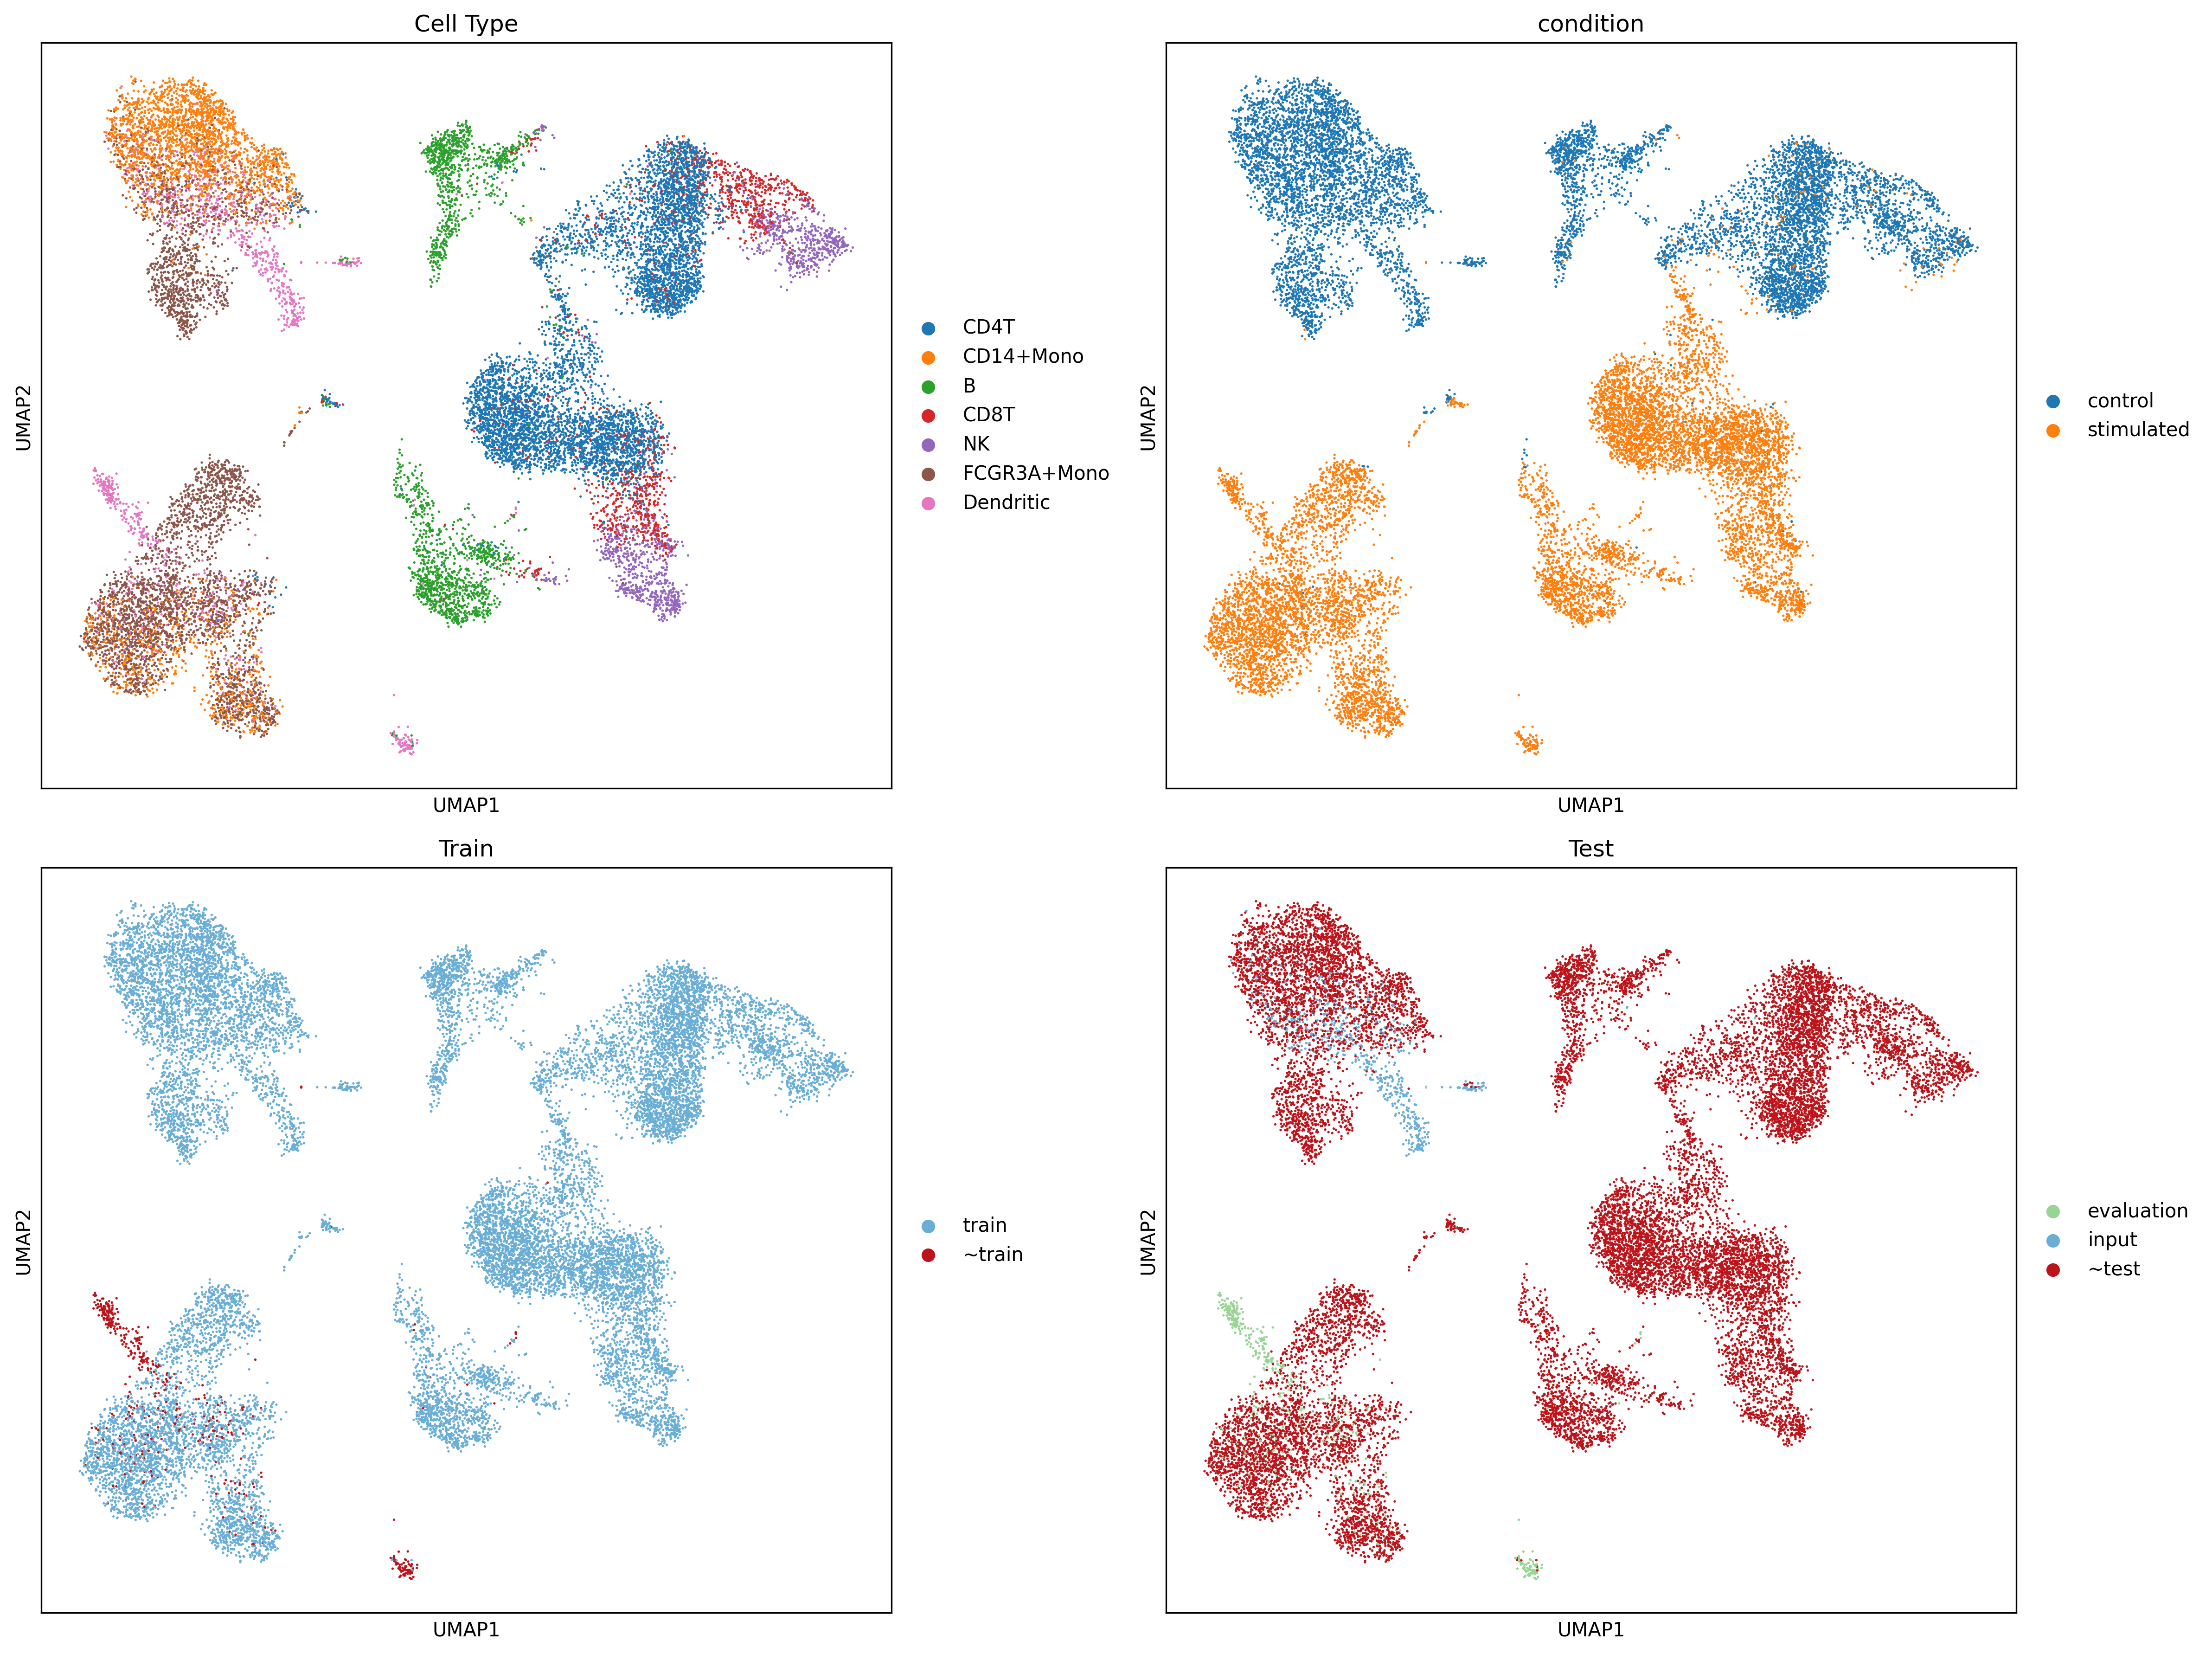
\includegraphics[width=0.9\textwidth]{figures/pbmc_split.png}
    \caption{Απεικόνιση UMAP του διαχωρισμού των δεδομένων (Kang et al. \cite{kanaGenerativeModelingSinglecell2023})}
    \label{fig:eval_pbmc_umap}
\end{figure}

\begin{figure}[h!]
    \centering
    \includegraphics[width=0.7\textwidth]{violins_pbmc.png}
    \caption{Διάγραμμα βιολιού των κατανομών έκφρασης του γονιδίου ISG15 (Kang et al. \cite{kanaGenerativeModelingSinglecell2023})}
    \label{fig:eval_pbmc_violins}
\end{figure}

\begin{table}[h!]
    \centering
    \scalebox{0.75}{
    \begin{tabularx}{\textwidth}{lXXXXXXXXX}
    \toprule
    model & DEGs & $R^2_{\text{HVG}}$ & $R^2_{\text{HVG20}}$ & $R^2_{\text{HVG100}}$ & Euc & Was & E-dist & MPD & MMD \\
    \midrule
    MTAe & \textbf{75.714} & 0.946 & 0.871 & 0.917 & 0.488 & 0.892 & 0.651 & 0.949 & 0.488 \\
    MTAeAdv & 72.381 & 0.961 & 0.955 & 0.948 & 0.202 & 0.604 & 0.429 & 0.800 & 0.202 \\
    MTAeAdvG & 65.905 & 0.917 & 0.878 & 0.901 & 0.504 & 0.828 & 0.681 & 0.909 & 0.504 \\
    MTAeOT & 41.190 & 0.657 & 0.668 & 0.648 & 0.811 & 0.947 & 0.883 & 0.963 & 0.811 \\
    MTAePlusOT & 37.190 & 0.670 & 0.674 & 0.657 & 0.810 & 0.951 & 0.880 & 0.966 & 0.810 \\
    MTVae & 69.095 & 0.942 & 0.954 & 0.928 & 0.261 & 0.621 & 0.499 & 0.800 & 0.261 \\
    MTVaeOT & 39.571 & 0.669 & 0.678 & 0.663 & 0.813 & 0.955 & 0.883 & 0.966 & 0.813 \\
    MTVaePlusOT & 30.619 & 0.661 & 0.670 & 0.655 & 0.821 & 0.958 & 0.888 & 0.968 & 0.821 \\
    scButterfly & 60.727 & 0.891 & 0.914 & 0.889 & 0.271 & \textbf{0.601} & 0.469 & \textbf{0.779} & 0.271 \\
    scGen & 32.143 & 0.910 & 0.872 & 0.870 & 0.627 & 0.909 & 0.765 & 0.946 & 0.627 \\
    scPreGAN & 35.750 & 0.771 & 0.857 & 0.799 & 0.499 & 0.690 & 0.682 & 0.851 & 0.499 \\
    vidrSingle & 25.536 & \textbf{0.970} & \textbf{0.971} & \textbf{0.961} & \textbf{0.182} & 0.606 & \textbf{0.408} & 0.797 & \textbf{0.182} \\
    \bottomrule
    \end{tabularx}}
    \caption{Μέσοι όροι σε όλους τους τύπους κυττάρων (Kang et al. \cite{kanaGenerativeModelingSinglecell2023})}
    \label{tab:eval_pbmc}
\end{table}



\subsection{Πρόβλεψη μονοκυτταρικών διαταραχών με πολλαπλές διαταραχές}
\label{sec:eval_multiple_perturbations}
Όπως αναφέρθηκε στην \crefwithname{sec:eval_single_perturbation}, οι multi-task αρχιτεκτονικές μας δεν μπόρεσαν να αξιοποιήσουν κοινή πληροφορία μεταξύ διαταραχών όταν στη διάθεση υπήρχε μόνο μία διαταραχή. Για μια πιο ρεαλιστική αξιολόγηση, δοκιμάσαμε τα μοντέλα στο σύνολο δεδομένων των Nault et al. \cite{nault2021single,nault2022benchmarking}, που περιλαμβάνει έντεκα τύπους κυττάρων εκτεθειμένους σε οκτώ διαφορετικές δοσολογίες TCDD σε ποντίκια.

Το σύνολο δεδομένων προεπεξεργάστηκε με το Scanpy \cite{wolf2018scanpy}: φιλτράραμε κύτταρα με λιγότερα από 500 συνολικά counts και λιγότερα από 720 εκφραζόμενα γονίδια, καθώς και γονίδια που εκφράζονται σε λιγότερα από 100 κύτταρα. Τα δεδομένα μετασχηματίστηκαν λογαριθμικά για πιο σταθερή εκπαίδευση και επιλέχθηκαν οι 5.000 πιο μεταβλητές μεταγραφές (HVG).

Κάθε επίπεδο δοσολογίας αντιμετωπίστηκε ως ξεχωριστή διαταραχή, με την κατάσταση ελέγχου ως βάση. Το conditioning σήμα για τις multi-task αρχιτεκτονικές είναι ένα one-hot διάνυσμα με εννέα διαστάσεις: ένα στοιχείο για κάθε από τις οκτώ δοσολογίες και ένα για την κατάσταση ελέγχου. Για την αξιολόγηση εκπαιδεύσαμε ξεχωριστό μοντέλο ανά τύπο κυττάρου, κρατώντας εκτός τα διαταραγμένα προφίλ του τύπου αυτού για δοκιμή. Το ίδιο μοντέλο χρησιμοποιήθηκε για προβλέψεις σε όλες τις δοσολογίες, εκμεταλλευόμενο την ικανότητα conditioning στην ταυτότητα της διαταραχής.

Αντίθετα, τα baseline μοντέλα που δεν υποστηρίζουν conditioning σε πολλαπλές διαταραχές απαιτούσαν την εκπαίδευση ξεχωριστού μοντέλου για κάθε δοσολογία. Εξαίρεση αποτελεί το scVIDR, που σχεδιάστηκε για να χειρίζεται πολλαπλά επίπεδα δοσολογίας μέσα σε ένα ενιαίο μοντέλο.

Συνοψίζοντας τα αποτελέσματα κατά μέσο όρο σε όλους τους τύπους κυττάρων και δοσολογίες (βλ. \cref{tab:eval_nault}), όπως και στην περίπτωση της \crefwithname{sec:eval_single_perturbation}, το multi-task μοντέλο \verb|MTAe| πέτυχε τον υψηλότερο μέσο αριθμό DEGs (~20). Το scGen εμφάνισε τα υψηλότερα $R^2$ σκορ αλλά με πολύ χαμηλό αριθμό DEGs, ενώ το scButterfly παρέμεινε ανταγωνιστικό σε όλες τις μετρικές. Οι παραλλαγές με optimal transport αποδείχθηκαν ικανές στις μετρικές απόστασης αλλά ασθενείς στις baseline μετρικές.

\clearpage

\begin{figure}[h!]
    \centering
    \includegraphics[width=0.9\textwidth]{selected_benchmarking_cell_type_baseline_metrics_nault.png}
    \caption{Βασικές μετρικές ανά τύπους κυττάρων (Nault et al. \cite{nault2021single,nault2022benchmarking})}
    \label{fig:eval_nault}
\end{figure}

\begin{figure}[h!]
    \centering
    \includegraphics[width=0.88\textwidth]{selected_benchmarking_cell_type_distance_metrics_nault.png}
    \caption{Μετρικές απόστασης ανά τύπο κυττάρου (Nault et al. \cite{nault2021single,nault2022benchmarking})}
    \label{fig:eval_nault_distance}
\end{figure}

\begin{figure}[h!]
    \centering
    \includegraphics[width=0.9\textwidth]{selected_benchmarking_doses_baseline_metrics_nault.png}
    \caption{Βασικές μετρικές ανά δοσολογίες (Nault et al. \cite{nault2021single,nault2022benchmarking})}
    \label{fig:eval_nault_doses_baseline}
\end{figure}

\begin{figure}[h!]
    \centering
    \includegraphics[width=0.9\textwidth]{selected_benchmarking_doses_distance_metrics_nault.png}
    \caption{Μετρικές απόστασης ανά δοσολογίες (Nault et al. \cite{nault2021single,nault2022benchmarking})}
    \label{fig:eval_nault_doses_distance}
\end{figure}

\begin{figure}[h!]
    \centering
    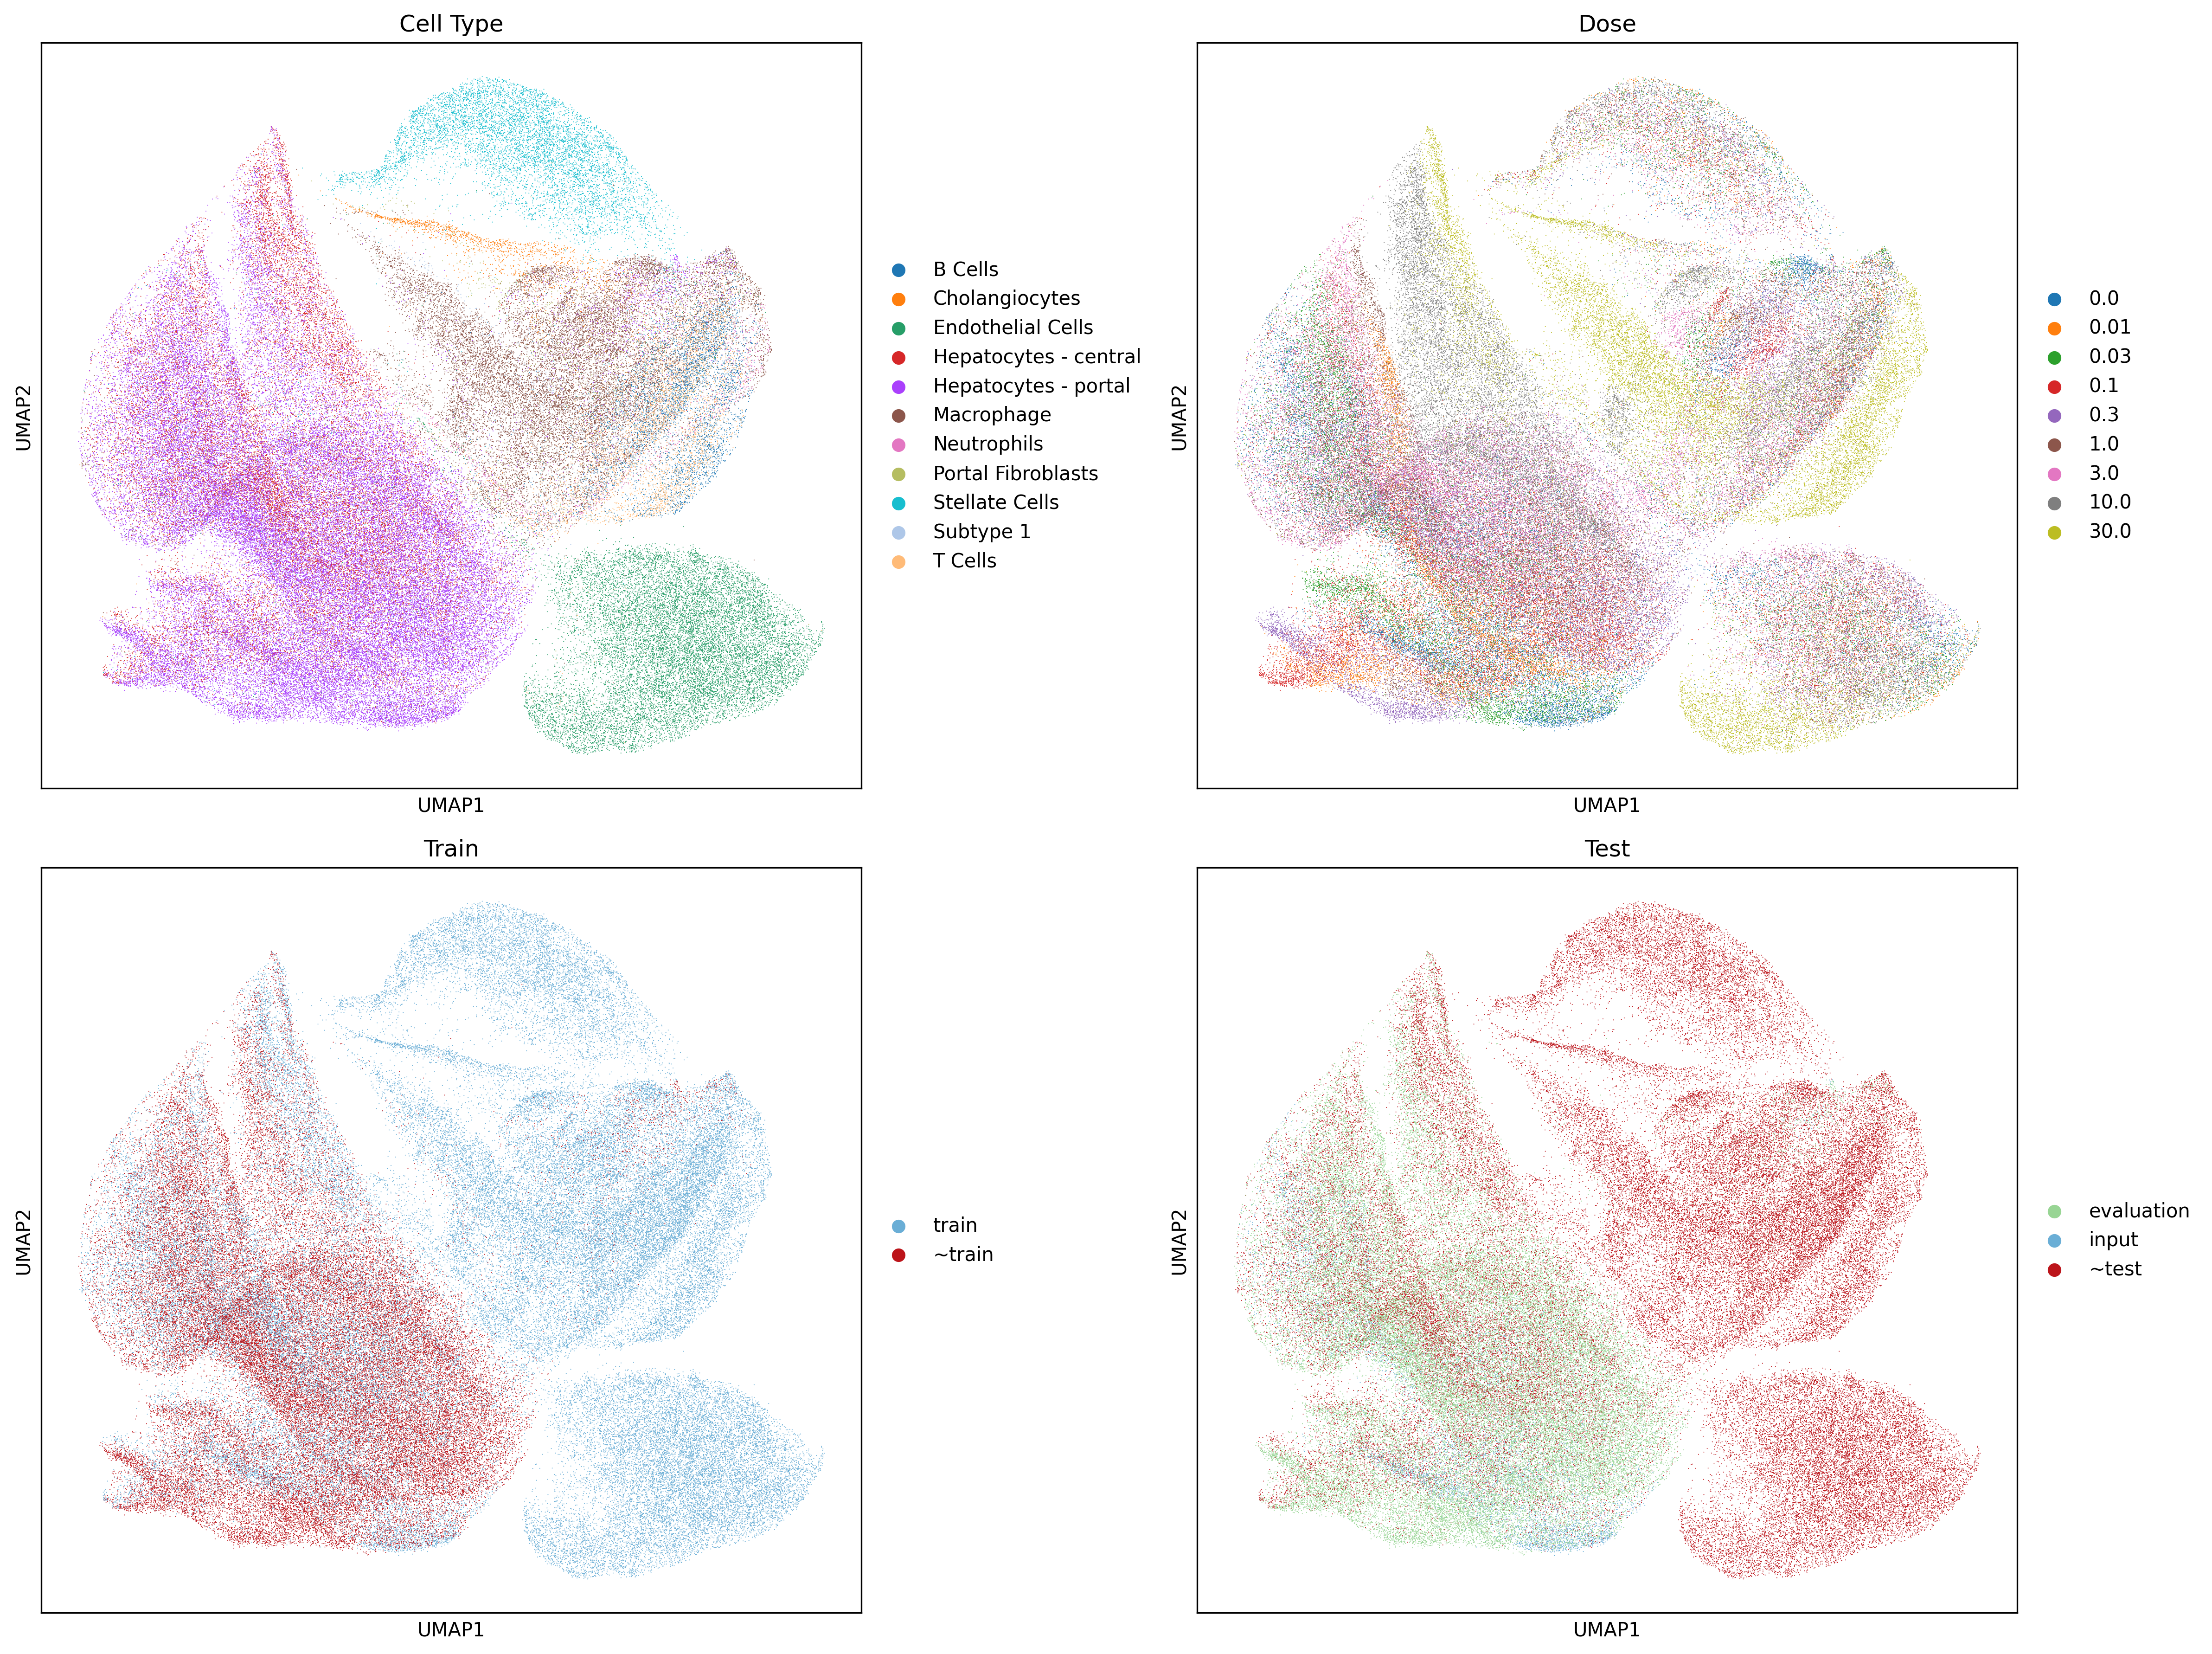
\includegraphics[width=0.85\textwidth]{figures/nault_umap_split_multiple.png}
    \caption{Απεικόνιση UMAP του διαχωρισμού των δεδομένων για όλες τις δοσολογίες (Nault et al. \cite{nault2021single,nault2022benchmarking})}
    \label{fig:eval_nault_umap_all}
\end{figure}

\begin{figure}[h!]
    \centering
    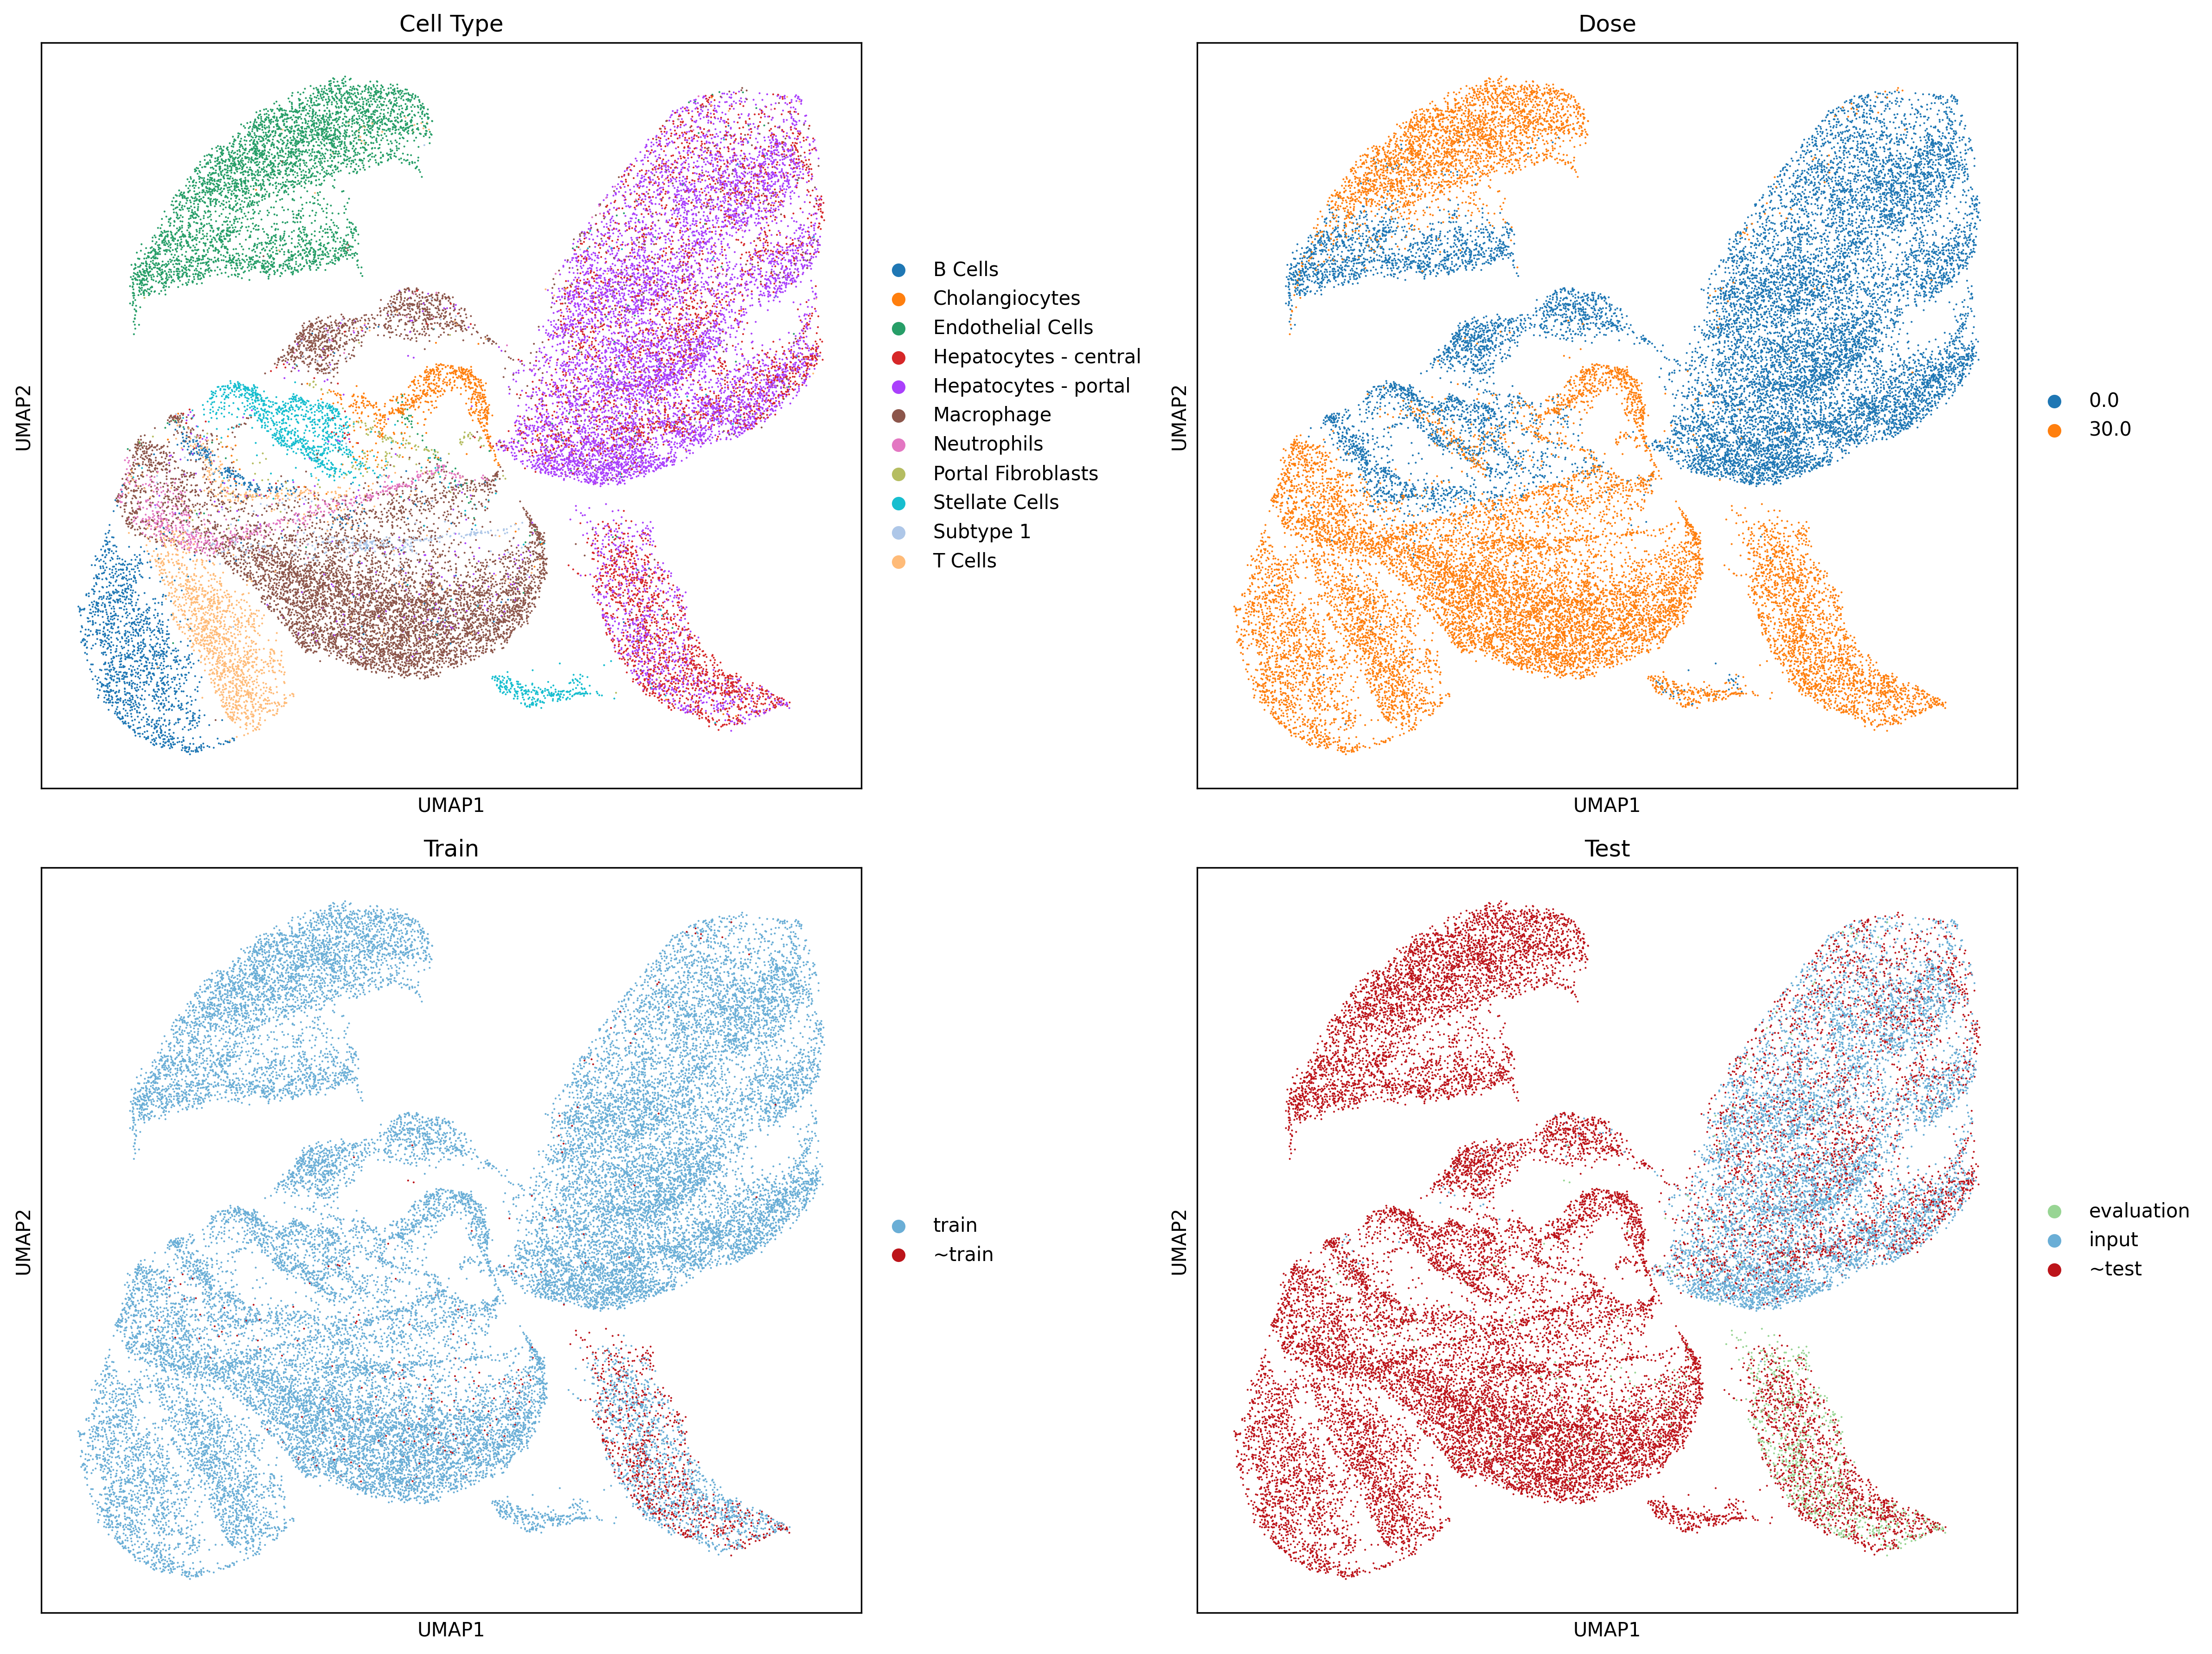
\includegraphics[width=0.85\textwidth]{figures/nault_umap_split_30.png}
    \caption{Απεικόνιση UMAP του διαχωρισμού των δεδομένων για τη δοσολογία $30 \mu g/kg$ (Nault et al. \cite{nault2021single,nault2022benchmarking})}
    \label{fig:eval_nault_umap_30}
\end{figure}


\begin{table}[h!]
    \centering
    \scalebox{0.75}{
    \begin{tabularx}{\textwidth}{lXXXXXXXXX}
    \toprule
    model & DEGs & $R^2_{\text{HVG}}$ & $R^2_{\text{HVG20}}$ & $R^2_{\text{HVG100}}$ & Euc & Was & E-dist & MPD & MMD \\
    \midrule
    MTAe & \textbf{20.341} & 0.862 & 0.792 & 0.833 & 1.386 & 1.217 & 1.116 & 1.050 & 1.386 \\
    MTAeAdv & 13.716 & 0.792 & 0.725 & 0.743 & 1.128 & 1.091 & 1.011 & 1.017 & 1.128 \\
    MTAeAdvG & 18.307 & 0.808 & 0.736 & 0.764 & 1.164 & 1.107 & 1.030 & 1.029 & 1.164 \\
    MTAeOT & 8.652 & 0.608 & 0.642 & 0.590 & 0.925 & 1.006 & 0.951 & 0.998 & 0.925 \\
    MTAePlusOT & 8.519 & 0.613 & 0.644 & 0.596 & \textbf{0.917} & \textbf{1.004} & 0.948 & 0.996 & 0.917 \\
    MTVae & 18.981 & 0.808 & 0.724 & 0.753 & 1.124 & 1.100 & 1.005 & 1.016 & 1.124 \\
    MTVaeOT & 8.163 & 0.614 & 0.642 & 0.593 & 0.929 & 1.009 & 0.952 & 0.998 & 0.929 \\
    MTVaePlusOT & 8.701 & 0.615 & 0.645 & 0.597 & 0.919 & 1.006 & 0.948 & 0.997 & \textbf{0.919} \\
    scButterfly & 16.818 & 0.740 & 0.694 & 0.696 & 0.984 & 1.014 & \textbf{0.944} & \textbf{0.990} & 0.984 \\
    scGen & 6.288 & \textbf{0.915} & \textbf{0.863} & \textbf{0.897} & 2.408 & 1.229 & 1.387 & 1.041 & 2.408 \\
    scPreGAN & 14.511 & 0.599 & 0.596 & 0.562 & 0.972 & 1.019 & 0.969 & 1.000 & 0.972 \\
    vidrMult & 2.352 & 0.870 & 0.837 & 0.852 & 9.295 & 1.358 & 2.425 & 1.054 & 9.295 \\
    vidrSingle & 3.795 & 0.855 & 0.797 & 0.824 & 1.431 & 1.174 & 1.118 & 1.025 & 1.431 \\
    \bottomrule
    \end{tabularx}}
    \caption{Nault et al. \cite{nault2021single,nault2022benchmarking}}
    \label{tab:eval_nault}
\end{table}



% \subsection{Cross-study}

% Robustness against batch effects is a critical aspect of generalization. To evaluate this, we assessed model performance across multiple studies, each potentially introducing technical variation due to differences in experimental protocols, platforms, or sample processing. This cross-study evaluation serves to test the ability of the models to generalize perturbation response predictions beyond dataset-specific biases. To implement this, similarly with the scGen's study, By holding out the perturbed profiles of a given study during training and evaluating the model on that study, we simulate an \gls{ood} setting with respect to study-level batch effects, thereby assessing the robustness and transferability of each approach across independently generated datasets.

\subsection{Πρόβλεψη μονοκυτταρικών διαταραχών μεταξύ ειδών}
\label{sec:eval_cross_species}


Μέχρι τώρα ο κύριος άξονας μεταβλητότητας για την αξιολόγηση της απόδοσης των μοντέλων ήταν η συνθήκη (control vs perturbed). Για να αξιολογήσουμε περαιτέρω την ανθεκτικότητα και τη γενίκευση των multi-task αρχιτεκτονικών εισάγουμε έναν επιπλέον άξονα μεταβλητότητας: το είδος (species).

Παρόμοια με την προσέγγιση της μελέτης scGen, χρησιμοποιήσαμε το σύνολο δεδομένων των Hagai et al. \cite{hagai2018gene}, το οποίο περιλαμβάνει μονοκυτταρικά προφίλ φαγοκυττάρων μυελού των οστών από τέσσερα είδη (ποντίκι, αρουραίο, κουνέλι και χοίρο), όλα υπό διέγερση με λιποπολυσακχαρίδη (LPS) για έξι ώρες.

Το σύνολο δεδομένων λήφθηκε προεπεξεργασμένο από τη μελέτη scGen. Για την αξιολόγηση ακολουθήσαμε την ίδια διαδικασία όπως στην \crefwithname{sec:eval_single_perturbation}, αλλά αντί να κρατήσουμε εκτός τα διαταραγμένα προφίλ ενός τύπου κυττάρου, κρατήσαμε εκτός τα διαταραγμένα προφίλ ενός είδους.

Συνοψίζοντας τα αποτελέσματα κατά μέσο όρο για όλα τα είδη (βλ. \cref{tab:eval_cross_species}), η \verb|MTAe| πέτυχε τον υψηλότερο μέσο αριθμό DEGs (~16). Τα scGen και scVIDR πέτυχαν τα υψηλότερα $R^2$ σκορ, όπως και στην περίπτωση της \crefwithname{sec:eval_single_perturbation}, αλλά είχαν χαμηλή απόδοση στις μετρικές απόστασης. Η \verb|MTVae| κατέγραψε την καλύτερη απόδοση στις μετρικές απόστασης και σχετικά υψηλό αριθμό DEGs (~12.5), αλλά χαμηλά $R^2$. Οι παραλλαγές με optimal transport τα πήγαν καλά στις μετρικές απόστασης αλλά ασθενώς στις baseline μετρικές, όπως και στο προηγούμενο σύνολο δεδομένων.

\begin{table}[h!]
    \centering    
    \scalebox{0.75}{
    \begin{tabularx}{\textwidth}{lXXXXXXXXX}
    \toprule
    model & DEGs & $R^2_{\text{HVG}}$ & $R^2_{\text{HVG20}}$ & $R^2_{\text{HVG100}}$ & Euc & Was & E-dist & MPD & MMD \\
    \midrule
    MTAe & \textbf{16.083} & 0.740 & 0.559 & 0.481 & 0.930 & 1.008 & 0.962 & 0.995 & 0.930 \\
    MTAeAdv & 11.250 & 0.579 & 0.465 & 0.365 & 0.865 & 0.919 & 0.929 & 0.957 & 0.865 \\
    MTAeAdvG & 12.500 & 0.708 & 0.533 & 0.456 & 0.921 & 0.985 & 0.958 & 0.987 & 0.921 \\
    MTAeOT & 7.500 & 0.483 & 0.432 & 0.304 & 0.899 & 0.932 & 0.948 & 0.966 & 0.899 \\
    MTAePlusOT & 8.000 & 0.480 & 0.436 & 0.309 & 0.876 & 0.913 & 0.936 & 0.956 & 0.876 \\
    MTVae & 12.500 & 0.652 & 0.498 & 0.413 & \textbf{0.840} & \textbf{0.903} & \textbf{0.916} & \textbf{0.951} & 0.840 \\
    MTVaeOT & 7.417 & 0.479 & 0.423 & 0.302 & 0.895 & 0.929 & 0.946 & 0.964 & 0.895 \\
    MTVaePlusOT & 7.833 & 0.473 & 0.431 & 0.301 & 0.883 & 0.919 & 0.940 & 0.959 & 0.883 \\
    scButterfly & 10.750 & 0.574 & 0.389 & 0.346 & 0.899 & 0.942 & 0.948 & 0.971 & 0.899 \\
    scGen & 7.583 & 0.826 & 0.705 & 0.658 & 2.014 & 1.576 & 1.367 & 1.165 & 2.014 \\
    scPreGAN & 7.250 & 0.443 & 0.374 & 0.276 & 0.914 & 0.945 & 0.955 & 0.973 & 0.914 \\
    vidrSingle & 12.917 & \textbf{0.878} & \textbf{0.711} & \textbf{0.701} & 3.386 & 1.905 & 1.769 & 1.225 & 3.386 \\
    \bottomrule
    \end{tabularx}}
    \caption{Hagel et al. \cite{hagai2018gene}}
    \label{tab:eval_cross_species}
\end{table}


\begin{figure}[h!]
    \centering
    \includegraphics[width=0.9\textwidth]{selected_benchmarking_cell_type_baseline_metrics_cross_species.png}
    \caption{Βασικές μετρικές ανά είδος (Hagai et al. \cite{hagai2018gene})}
    \label{fig:eval_cross_species}
\end{figure}

\begin{figure}[h!]
    \centering
    \includegraphics[width=0.9\textwidth]{selected_benchmarking_cell_type_distance_metrics_cross_species.png}
    \caption{Μετρικές απόστασης ανά είδος (Hagai et al. \cite{hagai2018gene})}
    \label{fig:eval_cross_species_distance}
\end{figure}


% \subsection{Overview}

% \begin{figure}[h!]
%     \centering
%     \includegraphics[width=\textwidth]{pcas.png}
%     \caption{PCA dimensionality reduction of the real unperturbed data, the real perturbed data and the predicted perturbed data.}
%     \label{fig:selected_nault_cell_type_baseline}
% \end{figure}

% scVIDR performance drops for DEGs, and distance metrics, but it performs well for the $R^2$ metrics and stays very consistent, along with scGEN. The multi-task models and scButterfly exhibit greater variability across measurements, but better performance on average. The optimal transport variations performed poorly overall, but were among the best for distance metrics for the Nault et al. \cite{nault2021single,nault2022benchmarking} dataset. 


\clearpage

\section{Συμπεράσματα και μελλοντικές προεκτάσεις της εργασίας}

Στην παρούσα εργασία προτείναμε μια αρχιτεκτονική μάθησης πολλαπλών εργασιών για τη μοντελοποίηση διαταραχών σε μονοκυτταρικά δεδομένα (\gls{sc}), ικανή να κάνει conditioning στον τύπο της διαταραχής. Ο σχεδιασμός αυτός επιτρέπει στο μοντέλο να αξιοποιεί κοινή πληροφορία μεταξύ διαφορετικών διαταραχών, οδηγώντας σε βελτίωση της απόδοσης στην εργασία πρόβλεψης εκτός κατανομής (\gls{ood}). Συγκρίναμε τα μοντέλα μας με τρέχουσες, state-of-the-art μεθόδους, όπως τα scGen, scVIDR, scPreGAN και scButterfly.

Επιπλέον, επιβεβαιώσαμε την προοπτική του scButterfly για τη μοντελοποίηση διαταραχών στο dataset πολλαπλών δοσολογιών των Nault et al. \cite{nault2021single,nault2022benchmarking}, επεκτείνοντας την αξιολόγηση πέρα από το σύνολο δεδομένων των Kang et al. \cite{kanaGenerativeModelingSinglecell2023} που χρησιμοποιήθηκε στην αρχική μελέτη.

Το βασικό μας μοντέλο, \verb|MTAe|, πέτυχε τον μεγαλύτερο αριθμό \gls{degs} σε όλα τα πειράματα (\crefwithname{sec:eval_single_perturbation}, \crefwithname{sec:eval_multiple_perturbations} και \crefwithname{sec:eval_cross_species}). Αν και κανένα μεμονωμένο μοντέλο δεν υπερέχει σταθερά σε όλες τις μετρικές, ένα σημαντικό πλεονέκτημα της multi-task προσέγγισης είναι η χαμηλότερη πολυπλοκότητα και η καλύτερη κλιμάκωση. Η μέθοδος απαιτεί την εκπαίδευση ενός μόνο μοντέλου ανά τύπο κυττάρου αντί για ένα μοντέλο ανά διαταραχή, όπως συμβαίνει στα baseline μοντέλα \cite{allenspachNeuralMultitaskLearning2024}. Αυτό καθιστά την προσέγγιση μας ιδιαίτερα συμφέρουσα για μεγάλα σύνολα δεδομένων με πολλές διαταραχές, μειώνοντας τόσο το υπολογιστικό κόστος όσο και τον χρόνο εκπαίδευσης. Μελλοντική εργασία θα μπορούσε να επικυρώσει περαιτέρω αυτή την αποδοτικότητα παραμέτρων εφαρμόζοντας την αρχιτεκτονική σε μεγαλύτερα και πιο ποικίλα σύνολα δεδομένων.

Μια περιορισμένη πτυχή της μεθόδου μας είναι ο εγγενώς transductive χαρακτήρας της όσον αφορά τις διαταραχές. Εφόσον το σήμα διαταραχής κωδικοποιείται ως one-hot, το μοντέλο δεν μπορεί να γενικεύσει σε μη παρατηρημένες διαταραχές. Μελλοντικές κατευθύνσεις θα πρέπει να εξετάσουν την ενσωμάτωση επαγωγικών (inductive) αναπαραστάσεων των διαταραχών στην αρχιτεκτονική μας, ώστε να επιτραπεί η εξωστρέφεια (extrapolation) σε νέα, μη παρατηρημένα perturbations.

% we could explore to apply a combination of perturbations as well

\clearpage

\section{Διαθεσιμότητα κώδικα}

Ο κώδικας για τα μοντέλα και τα πειράματα είναι διαθέσιμος στο \url{https://github.com/thodkatz/thesis}.

\clearpage


\addcontentsline{toc}{section}{References}
\bibliographystyle{plain}
\bibliography{../references.bib}

\clearpage


\addcontentsline{toc}{section}{Παράρτημα}
\section*{Παράρτημα Α}


\addcontentsline{toc}{subsection}{Α. Πρόσθετη αξιολόγηση των αρχιτεκτονικών με μάθηση πολλαπλών εργασιών}
\subsection*{Πρόσθετη αξιολόγηση των αρχιτεκτονικών με μάθηση πολλαπλών εργασιών}
\label{sec:appendix_evaluation}

\begin{figure}[h!]
    \centering
    \includegraphics[width=0.77\textwidth]{multi_task_benchmarking_cell_type_baseline_metrics_pbmc.png}
    \caption{Βασικές μετρικές ανά τύπο κυττάρου (Kang et al. \cite{kang2018multiplexed})}
    \label{fig:all_multi_task_kang}
\end{figure}

\begin{figure}[h!]
    \centering
    \includegraphics[width=0.77\textwidth]{multi_task_benchmarking_cell_type_distance_metrics_pbmc.png}
    \caption{Μετρικές απόστασης ανά τύπο κυττάρου (Kang et al. \cite{kang2018multiplexed})}
    \label{fig:all_multi_task_kang_distance}
\end{figure}

\begin{figure}[h!]
    \centering
    \includegraphics[width=0.9\textwidth]{multi_task_benchmarking_cell_type_baseline_metrics_nault.png}
    \caption{Βασικές μετρικές ανά τύπο κυττάρου (Nault et al. \cite{nault2021single,nault2022benchmarking})}
    \label{fig:all_multi_task_nault}
\end{figure}

\begin{figure}[h!]
    \centering
    \includegraphics[width=0.9\textwidth]{multi_task_benchmarking_cell_type_distance_metrics_nault.png}
    \caption{Μετρικές απόστασης ανά τύπο κυττάρου (Nault et al. \cite{nault2021single,nault2022benchmarking})}
    \label{fig:all_multi_task_nault_distance}
\end{figure}

\begin{figure}[h!]
    \centering
    \includegraphics[width=0.9\textwidth]{multi_task_benchmarking_doses_baseline_metrics_nault.png}
    \caption{Βασικές μετρικές ανά δοσολογίες (Nault et al. \cite{nault2021single,nault2022benchmarking})}
    \label{fig:all_multi_task_nault_doses_baseline}
\end{figure}

\begin{figure}[h!]
    \centering
    \includegraphics[width=0.9\textwidth]{multi_task_benchmarking_doses_distance_metrics_nault.png}
    \caption{Μετρικές απόστασης ανά δοσολογίες (Nault et al. \cite{nault2021single,nault2022benchmarking})}
    \label{fig:all_multi_task_nault_doses_distance}
\end{figure}

\end{document}